\documentclass[12pt, letterpaper, preprint, tighten]{aastex62}
%\usepackage[breaklinks,colorlinks, urlcolor=blue,citecolor=blue,linkcolor=blue]{hyperref}
%\usepackage{hyperref}
\usepackage{amsmath}
\usepackage{color}
\usepackage{comment}

% typesetting shih
\linespread{1.08} % close to 10/13 spacing
\setlength{\parindent}{1.08\baselineskip} % Bringhurst
\setlength{\parskip}{0ex}
\let\oldbibliography\thebibliography % killin' me.
\renewcommand{\thebibliography}[1]{%
  \oldbibliography{#1}%
  \setlength{\itemsep}{0pt}%
  \setlength{\parsep}{0pt}%
  \setlength{\parskip}{0pt}%
  \setlength{\bibsep}{0ex}
  \raggedright
}
\setlength{\footnotesep}{0ex} % seriously?

\definecolor{orange}{rgb}{1,0.5,0}
\definecolor{dred}{rgb}{0.59,0.,0.09}

\newcommand\tab[1][1cm]{\hspace*{#1}}
\newcommand{\ch}[1]{{\color{orange}{\bf CH:} #1}}
\newcommand{\edt}[1]{{\color{dred}{\bf} #1}}
\newcommand{\beq}{\begin{equation}}
\newcommand{\eeq}{\end{equation}}
\newcommand{\overbar}[1]{\mkern 1.5mu\overline{\mkern-1.5mu#1\mkern-1.5mu}\mkern 1.5mu}
\newcommand{\avgSFR}{\overline{\raisebox{0pt}[1.2\height]{SFR}}}
\newcommand{\cao}{Cao et al. (in preparation)}
\newcommand{\SFR}{\mathrm{SFR}}
\newcommand{\fq}{f_\mathrm{Q}}
\newcommand{\fqcen}{f_\mathrm{Q}^\mathrm{cen}}
\newcommand{\zinit}{z_\mathrm{initial}}
\newcommand{\taucen}{\tau_\mathrm{Q}^\mathrm{cen}}
\newcommand{\tduty}{t_{\rm duty}}
\newcommand{\logsfr}{\log\mathrm{SFR}}
\newcommand{\logsfrsfs}{\log\mathrm{SFR}_\mathrm{SFS}}
\newcommand{\bitem}{\begin{itemize}}
\newcommand{\eitem}{\end{itemize}}
\newcommand{\musfms}{\log\overline{\mathrm{SFR}}_\mathrm{SFS}}
\newcommand{\siglogm}{\sigma_{\log M_*}}

\begin{document}\sloppy\sloppypar\frenchspacing

%\title{The Star-Forming Sequence in a Hierarchical Universe}
\title{Star Formation Histories of Star Forming Galaxies in a Hierarchical Universe}
\author{ChangHoon Hahn}
\altaffiliation{hahn.changhoon@gmail.com}
\affil{Lawrence Berkeley National Laboratory, 1 Cyclotron Rd, Berkeley CA 94720, USA}
\affil{Berkeley Center for Cosmological Physics, University of California, Berkeley, CA 94720, USA}
\affil{Center for Cosmology and Particle Physics, Department of Physics, New York University, 4 Washington Place, New York, NY 10003}
\author{Jeremy L.~Tinker}
\affil{Center for Cosmology and Particle Physics, Department of Physics, New York University, 4 Washington Place, New York, NY 10003}
\author{Andrew R.~Wetzel}
\affil{TAPIR, California Institute of Technology, Pasadena, CA USA}
\affil{Carnegie Observatories, Pasadena, CA USA}
\affil{Department of Physics, University of California, Davis, CA USA}

\begin{abstract}
    We present constraints on the timescale of star formation variability and the 
    correlation between star formation and host halo accretion histories of star-forming
    central galaxies. Star-forming galaxies are found to have a tight relationship
    between their star formation rates and stellar masses on the so-called ``star-forming
    sequence'' (SFS), which characterizes both their star formation histories and
    stellar mass growths. Meanwhile, observed constraints on the stellar-to-halo
    mass relation (SHMR) connect stellar mass growth to host halo halo accretion
    history. Combining these observed trends with a high-resolution cosmological
    $N$-body simulation, we present flexible models that track the star formation,
    stellar mass, and host halo accretion histories of star-forming central galaxies
    over $z < 1$. We then compare this model to the observed stellar mass function
    and SFS of central galaxies in SDSS Data Release 7 to find that the scatter
    in SHMR at $M_h{=}10^{12}M_\odot$, $\sigma_{\log M_*}$, is sensitive to the
    timescale of star formation variability, $t_{\rm duty}$, and the correlation 
    coefficient, $r$, between star formation and host halo accretion histories. 
    Variations on shorter timescales produce tighter $\sigma_{\log M_*}$; higher 
    $r$ also produce tighter scatter in the SHMR. We find that a correlation of 
    $r > 0.5$ and $t_{\rm duty} \leq 1$ Gyr is necessary to reproduce the constant 
    $\sigma_{\log M_*} \sim 0.2$ dex over $z=1$ to 0, as found in halo model based 
    observational constraints and hydrodynamic simulations. For $r \sim 0.6$ 
    constraints found in the literature, $t_{\rm duty} < 0.5$ Gyr is necessary. 
    \ch{need a sentence on the higher and decreasing $\siglogm(z\sim1)$ and what 
    that tells us.}
    The lack of consensus among the SHMRs of observations and galaxy formation models,
    however, remains the primary bottleneck in precisely constraining $r$ and
    $t_\mathrm{duty}$. Nevertheless, we demonstrate that SHMR can be used to 
    constrain star formation and halo accretion histories.
\end{abstract}
\keywords{methods: numerical -- galaxies: evolution -- galaxies: haloes --
galaxies: star formation -- galaxies: groups: general -- cosmology: observations.}

%Observations also place constraints on the stellar-to-halo mass relation (SMHR), which suggest that  the evolution of star forming galaxies is also inextricably linked to the underlying halo.
%The SFS alone, however, does not dictate the evolution star forming galaxies.
%Based on observed constraints on the stellar-to-halo mass relation (SHMR), halo  accretion history also likely plays a role in the evolution  of star-forming galaxies.
%By combining a high-resolution cosmological $N$-body  simulation with observed evolutionary trends of the SFS, we present a model that  tracks the star formation, stellar mass, and host halo mass histories of  star-forming central galaxies over $z < 1$ and

\section{Introduction}
Observations from large surveys such as the Sloan Digital Sky Survey~\citep[SDSS;][]{york2000}
have been critical for establishing the global trends of galaxies in
the local universe. Broadly speaking, galaxies fall into two categories:
quiescent and star-forming (hereafter SF) galaxies. Quiescent galaxies
have little to no star formation, are red in color
\edt{due to old stellar populations},
and have ellipitical
morphologies. Meanwhile, SF galaxies have significant star formation,
\edt{thus}
are blue in color, and have disk-like morphologies (\citealt{kauffmann2003, blanton2003, baldry2006, taylor2009, moustakas2013};
see~\citealt{blanton2009} and references therein).
SF galaxies, furthermore, are found on the so-called ``star-forming sequence''
(hereafter SFS), a tight relationship between their star formation rates (SFR)
and stellar masses~\citep[][see also Figure~\ref{fig:groupcat}]{noeske2007, daddi2007, salim2007, speagle2014, lee2015}.
This sequence, which is observed out to $z > 2$~\citep{wang2013, leja2015}
plays a crucial role in
\edt{determining}
galaxy evolution over the past ${\sim}10\,\mathrm{Gyr}$~\citep[see][for an alternative point of view]{kelson2014,abramson2016}.
The significant fraction of SF galaxies that quench their
star formation and migrate off of the SFS reflects the growth in the
fraction of quiescent galaxies~\citep{blanton2006, borch2006, bundy2006, moustakas2013}.
The decline of star formation in the entire SFS~\citep{lee2015, schreiber2015}
over time reflects the decline in overall cosmic star formation~\citep{hopkins2006, behroozi2013, madau2014}.
With its evolution, the SFS also connects the star formation histories of SF
galaxies to their stellar mass growths.

These observations have also allowed us to investigate how galaxies fit
into the context of hierarchical structure formation predicted by 
$\Lambda$CDM cosmology. In addition to traditional theoretical
models of hydrodynamic simulations and semi-analytic
models~\citep[see][for reviews]{silk2012, somerville2015},
empirical models 
\edt{have been remarkably effective} 
for understanding the galaxy-halo connection. These models relate galaxy
properties to their host dark matter halo properties using methods such as
halo occupation distribution modeling~\citep[HOD; \emph{e.g.}][]{zheng2007,zehavi2011,leauthaud2012,parejko2013,zu2015},
\edt{conditional} luminosity function modeling~\citep[\emph{e.g.}][]{yang2009}, and abundance
matching~\citep[\emph{e.g.}][]{kravtsov2004, vale2006, conroy2009, moster2013, reddick2013}.
Using these models, we find that more massive halos host more
massive galaxies with a tight scatter in the stellar-to-halo
mass relation~\citep[hereafter SHMR;][]{mandelbaum2006a, conroy2007, more2011, leauthaud2012, tinker2013, velander2014, han2015, zu2015, gu2016, lange2018a}. 
An equally tight SHMR is found at higher
$z\sim1$~\citep{leauthaud2012, tinker2013, patel2015}. This lack of
evolution in the scatter of the SHMR suggests that stellar
mass growth of galaxies is linked somehow to the growth
of their host dark matter halos.

Despite these developments, we face a number of challenges when it comes
to understanding the detailed star formation histories (SFH) and its
connection to host halo assembly history of galaxies.
For instance, SFHs at lookback times longer than $200\,\mathrm{Myr}$
do not contribute to SFR indicators such as $H\alpha$ or $FUV$ fluxes~\cite{sparre2017}.
Measuring SFHs from fitting photometry or spectroscopy typically
assume a specific functional form of the SFH, such as exponentially
declining or lognormal, that do not include variations on short
timescales~\citep[\emph{e.g.}][]{wilkinson2017, carnall2018}.
Even methods that recover non-parametric SFHs from high signal-to-noise
observations can only retrieve SFHs in coarse temporal resolutions~\citep[\emph{e.g.}][]{tojeiro2009, leja2018a}.
While simulations provide another means for understanding SFHs,
they are also subject to their specific time and mass resolutions that
suppress the variability of their star formation, especially in
analytic models, semi-analytic models, and large-volume cosmological
hydrodynamic simulations~\citep[][see also Figure~\ref{fig:illsfh}]{sparre2015, sparre2017}.

Empirical models, \edt{through their} flexibility, provide an effective 
method for examining the connection between SFH and host halo assembly 
history. A number of empirical models~\citep{taghizadeh-popp2015, becker2015, rodriguez-puebla2016a, mitra2017, cohn2017, moster2017},
relate SFHs of galaxies linearly to their host halo mass accretion
rates and successfully reproduce a number of observations. Such models
make the strong assumption that SFH of galaxies are perfectly 
correlated to halo accretion history. 
\edt{Recently by analyzing the observed correlation between the SFRs 
and large-scale environment of SF galaxies, \cite{tinker2018b} found the 
first observational evidence that this is true, but with a correlation 
coefficient of only $r \sim 0.63$.}
These models, therefore, ignore variation in star formation independent 
from halo accretion, which may come from physical processes in galaxies. 
More recently, the empirical model of \cite{behroozi2018} correlate SFH
with halo assembly while also incorporating star formation variability in
the SFH. For halos at a given $v_{\rm M_{peak}}$ (the maximum circular
velocity of the halo at the redshift of max halo mass) and $z$, they
assign higher SFRs to halos with higher values of $\Delta v_{\rm max}$
(logarithmic growth in the maximum circular velocity of the halo over past dynamical time)
allowing for random scatter in the assignment. Through this random scatter,
which is further separated into contributions from shorter and longer timescales,
they incorporate star formation variability. Explicitly examining and constraining
the timescale of star formation variability, however, is difficult with such a
parameterization.

Constraints on the timescale of star formation variability can be used to
shed light on physical processes involved in galaxy star formation and
constrain galaxy feedback models~\citep{sparre2015}. For instance,
it can be used to differentiate between physical processes such
as galactic feedback interacting with the circumgalactic medium, which
would cause longer timescale variations, or internal processes affecting
the cold gas in the galaxy, which would cause $\sim 100$ Myr variations.
Using the Feedback In Realistic Environments (FIRE) high resolution
cosmological simulations, \cite{hopkins2014} find that
explicit and resolved feedback increases time varaibility in SFRs.
Also using FIRE, \cite{sparre2017} find that varying the strength of
Type II supernova feedback can change the burstiness of SFHs.
\cite{governato2015} find that HI shielding from UV radiation and
early feedback from young stars would also produce small scale star
formation variability.

\edt{In this paper, we construct empirical models to investigate the timescale
of star formation varability and the connection between SFH and host halo
accretion history of SF central galaxies. 
Central galaxies constitute the majority of massive galaxies ($M_*>10^{9.5}M_\sun$) 
at $z\sim0$~\citep{wetzel2013} and their SFHs are not influenced by 
environmentally-driven external mechanisms such as ram pressure 
stripping~\citep{gunn1972,bekki2009}, strangulation~\citep{larson1980, peng2015}, or 
harassment~\citep{moore1998} that impact SFHs of satellites. 
}
Using a similar approach as \cite{wetzel2013, hahn2017b}, we present models
that combine a high resolution cosmological $N$-body simulation with
observed evolutionary trends of the SFS. They statistically track the 
star formation, stellar mass, and host halo assembly histories of SF central 
galaxies over $z\sim1$ to $0$. Comparing predictions of our empirical models 
to properties of observed galaxies and observational constraints on the SHMR 
allows us to constrain the timescale of star formation variability and the 
correlation between SFH and host halo assembly history. 
\edt{More specifically, we present the constraints derived from the observed 
tight scatter of the SHMR, $\siglogm\sim0.2$ dex, and its lack of evolution 
over $z\sim1$ to $0$ as found in halo model analyses mentioned earlier. These 
halo model analyses, however, mainly constrain $\siglogm$ at high halo masses 
($M_h > 10^{12}M_\odot$). At lower halo masses, there is no clear consensus 
among observational constraints. However, in the recent \cao analysis, they find, 
using a more direct measurement, larger scatter $\siglogm(M_h\sim 10^{12} M_\odot) \sim 0.3$ 
dex from observations. They also find that in the Illustris TNG~\citep{pillepich2018} 
hydrodynamic simulation, $\siglogm(M_h\sim 10^{12} M_\odot)$ decreases from 
$z=1$ to $0$. We, therefore, also present the timescale of star formation variability 
and the correlation between SFH and host halo assembly history for larger 
$\siglogm$ that decreases over cosmic time. 
}

%In this paper, we construct an empirical model of SF central galaxies,
%the timescale of star formation variability in their
%SFH, and the connection between their SFH and host halo accretion history.
%We focus on central galaxies since the SFHs of satellites are influenced
%by environmentally-driven external mechanisms such as ram pressure
%stripping~\citep{gunn1972,bekki2009}, strangulation~\citep{larson1980, peng2015},
%or harassment~\citep{moore1998}. Moreover, centrals constitute the majority
%of massive galaxies ($M_*>10^{9.5}M_\sun$) at $z\sim0$~\citep{wetzel2013}.
%Using a similar approach as \cite{wetzel2013, hahn2017b}, we present a model
%that combines a high resolution cosmological $N$-body simulation with
%observed evolutionary trends of the SFS. Our model statistically tracks
%the star formation, stellar mass, and host halo assembly histories of SF
%central galaxies over $z\sim1$ to $0$. By comparing predictions of this empirical
%model to observations, in particular measurements of the scatter in the
%SHMR, we constrain the timescale of star formation variability and also
%the correlation between SFH and host halo assembly history.

In Section~\ref{sec:sdss} we describe the $z\approx0$ central galaxy
sample that we construct from SDSS Data Release 7. Then in
Section~\ref{sec:sim}, we describe the $N$-body simulation and how we
evolve the SFR and stellar masses of the star-forming central galaxies
in our model. We compare predictions from our model to observations
and present the resulting constraints in Section~\ref{sec:results}.
Finally, we conclude and summarize the results in Section~\ref{sec:summary}.
%%%%%%%%%%%%%%%%%%%%%%%%%%%%%%%%%%%%%
% Figure 1
%%%%%%%%%%%%%%%%%%%%%%%%%%%%%%%%%%%%%
\begin{figure}
\begin{center}
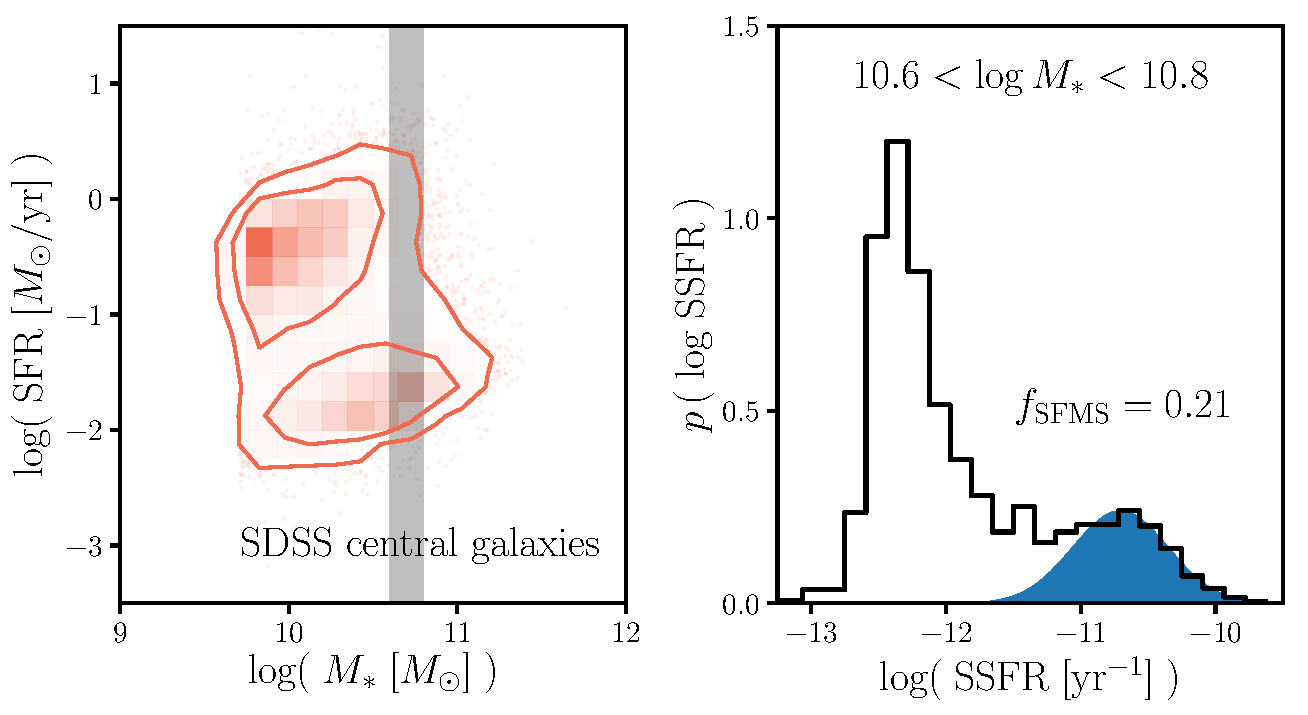
\includegraphics[width=0.75\textwidth]{figs/groupcat.pdf}
    \caption{The SFR--$M_*$ relation of the central galaxies in SDSS DR7
    mark the bimodal distribution of the star-forming and quiescent
    populations (left panel). \emph{Star-forming centrals, based on the correlation between their
    SFR and $M_*$, lie on the so-called ``star-forming sequence''}.
    %The transitioning galaxies lie on the ``green'' valley between the star-fomring and quiescent modes.
    On the right, we present the SSFR distribution, $p(\log\mathrm{SSFR})$,
    of SDSS centrals with $10.6 < \log M_* < 10.8$. Based on the SFS component
    from the \cite{hahn2018a} GMM fit to the SFR--$M_*$ relation (shaded in blue),
    galaxies in the SFS account for $f_\mathrm{SFS} = 0.21$ of the centrals
    in the stellar mass bin.} \label{fig:groupcat}
\end{center}
\end{figure}
%%%%%%%%%%%%%%%%%%%%%%%%%%%%%%%%%%%%%

\section{Central Galaxies of SDSS DR7} \label{sec:sdss}
We construct our galaxy sample following the sample selection of \cite{tinker2011}.
We select a volume-limited sample of galaxies at $z \approx 0.04$ with
$M_r - 5 \log(h) < -18$ and complete above $M_* > 10^{9.4} h^{-2}M_\odot$ from
the NYU Value-Added Galaxy Catalog \citep[VAGC;][]{blanton2005} of the
Sloan Digital Sky Survey Data Release 7~\citep[SDSS DR7;][]{abazajian2009}.
The stellar masses of these galaxies are estimated using the
$\mathtt{kcorrect}$ code~\citep{blanton2007} assuming a~\cite{chabrier2003}
initial mass function. For their specific star formation rates (SSFR) we use
measurements from the current release of the MPA-JHU spectral
reductions\footnote{http://wwwmpa.mpa-garching.mpg.de/SDSS/DR7/}~\citep{brinchmann2004}.
Generally, $\mathrm{SSFR} > 10^{-11}\mathrm{yr}^{-1}$ are derived from
$\mathrm{H}\alpha$ emission, $10^{-11} > \mathrm{SSFR} > 10^{-12}\mathrm{yr}^{-1}$
are derived from a combination of emission lines, and $\mathrm{SSFR} < 10^{-12}\mathrm{yr}^{-1}$
are based on $D_n 4000$~\citep[see discussion in][]{wetzel2013}. We emphasize that
$\mathrm{SSFR} < 10^{-12}\mathrm{yr}^{-1}$ should only be considered upper limits
to the actual galaxy SSFR~\citep{salim2007}.

From this galaxy sample, we identify central galaxies using the
\cite{tinker2011} group finder, a halo-based algorithm that uses
the abundance matching ansatz to iteratively assign halo masses to
groups~\edt{\citep[see also][]{yang2005}}.
It assigns an initial halo mass to each galaxy by matching their
abundances. Then starting with the most massive galaxy, nearby lower
mass galaxies are assigned a probability of being a satellite. Once all
the galaxies are assigned to a group, the halo masses of the central galaxies
are updated by abundance matching with the total stellar mass in the groups.
This entire process is repeated until convergence. Every group contains one
central galaxy, which by definition is the most massive, and a group can
contain zero, one, or many satellites.
%\todo{The algorithm assigns a probability of being a satellite, $P_\mathrm{sat}$, to each galaxy in the sample. Galaxies with $P_\mathrm{sat} \geq 0.5$  are classified as satellites and $P_\mathrm{sat} < 0.5$ are classified as centrals.} In this paper we focus on central galaxies.
As with any group finder, galaxies are misassigned due to projection
effects and redshift space distortions. Our central galaxy sample has
a purity of ${\sim}90\%$ and completeness of ${\sim}95\%$~\citep{tinker2018}
Moreover, as illustrated in \cite{campbell2015}, the \cite{tinker2011} group
finder robustly identifies red and blue centrals as a function of stellar mass,
which is highly relevant to our analysis.
We present the SFR--$M_*$ relation of the SDSS DR7 central galaxies, described
above, in the left panel of Figure~\ref{fig:groupcat}. The contours of the
relation clearly illustrate the bimodality in the galaxy sample with the
star-forming centrals lying on the so-call ``star-forming sequence'' (SFS).
% In the left panel of Figure~\ref{fig:groupcat}, we plot the SFR-$M_*$ distribution of the SDSS DR7 central galaxies. In the right panel, we plot the distribution of SSFR,  $p(\log \mathrm{SSFR})$, for galaxies with $10.6 < \log \,M_* < 10.8$ (stellar mass range  highlighted on the left panel). Both panels of Figure~\ref{fig:groupcat} illustrate the  bimodality in the galaxy sample. The SFR-$M_*$ distribution also illustrate the correlation between SFR and $M_*$ in star-forming galaxies \emph{i.e.} the star-formation main sequence  (SFS).

\section{Model: Simulated Central Galaxies} \label{sec:sim}
\edt{We are} interesting in constructing a model that tracks central galaxies and
their star formation within the heirarchical growth of their host halos. This
requires a cosmological $N$-body simulation that accounts for the complex
dynamical processes that govern the host halos of galaxies. In this paper
we use the high resolution $N$-body simulation from~\cite{wetzel2013} generated
using the \cite{white2002} $\mathtt{TreePM}$ code with flat $\Lambda$CDM cosmology
($\Omega_m =0.274, \Omega_b = 0.0457, h = 0.7, n=0.95$, and $\sigma_8 = 0.8$).
From initial conditions at $z = 150$, generated from second-order Lagrangian
Perturbation Theory, $2048^3$ particles with mass of $1.98 \times 10^8\,M_\odot$ are
evolved in a \edt{$250\,h^{-1}\mathrm{Mpc}$} box with a Plummer equivalent smoothing of
\edt{$2.5\,h^{-1}{\rm kpc}$}~\citep{wetzel2013, wetzel2014}. `Host halos' are then
identified using the Friends-of-Friends algorithm~\citep[FoF;][]{davis1985} with
linking length of $b{=}0.168$ times the mean inter-partcile spacing. Within
these host halos, \cite{wetzel2013} identifies `subhalos' as overdensities
in phase space through a six-dimensional FoF algorithm~\citep[FoF6D;][]{white2010}.
The host halos and subhalos are then tracked across the simulation outputs
from $z = 10$ to $0$ to build merger trees~\citep{wetzel2009,wetzel2010}.
The most massive subhalos in newly-formed host halos at a given simulation
output are defined as the `central' subhalo. A central subhalo retains its
`central' definition until it falls into a more massive host halo
\edt{(FoF halo mass)}, at which point it becomes a `satellite' subhalo.

Throughout its $45$ snapshot outs, $\mathtt{TreePM}$ simulation tracks
the evolution of subhalos back to $z \sim 10$. We restrict ourselves to $15$
snapshots from $z = 1.08$ to $0.05$, where we have the most statistically
meaningful observations. Furthermore, since we're interested in centrals we only
keep subhalos that are classified as centrals throughout the redshift
range. This criterion removes ``black splash'' or ``ejected'' satellite
galaxies~\citep[\emph{e.g.}][]{mamon2004,wetzel2014} misclassified as
centrals. Next, we describe how we select and initialize the SF central
galaxies from the central subhalos of the $\mathtt{TreePM}$
simulation in our model.

%%%%%%%%%%%%%%%%%%%%%%%%%%%%%%%%%%%%%%%%%%%%%%%%%%%%%%%%%%%%%%%%%%%%%%%%%%
% Section
%%%%%%%%%%%%%%%%%%%%%%%%%%%%%%%%%%%%%%%%%%%%%%%%%%%%%%%%%%%%%%%%%%%%%%%%%%
\subsection{Selecting Star-Forming Centrals}  \label{sec:sfcen}
To construct a model that tracks the SFR and stellar mass evolution of
star-forming central galaxies, we first need to select them from the
central galaxies/subhalos in the $\mathtt{TreePM}$ simulation. Since
we want our model to reproduce observations, our selection is based
on $f^\mathrm{cen}_\mathrm{SFS}(M_*)$, the fraction of central galaxies
within the SFS measured from the SDSS DR7 VAGC (Section~\ref{sec:sdss}).
Below, we describe how we derive $f^\mathrm{cen}_\mathrm{SFS}(M_*)$ and
use it to select SF central galaxies in our model. Afterwards
we describe how we initialize the SFRs and $M_*$ of these galaxies at
$z = 1$.

Often in the literature, an empirical color-color or SFR--$M_*$ cut
that separates the two main modes (red/blue or star-forming/quiescent)
in the distribution is chosen to classify
galaxies~\citep[\emph{e.g.}][]{baldry2006, blanton2009, drory2009, peng2010, moustakas2013, hahn2015}.
The red/quiescent or blue/star-forming fractions derived from this sort
of classification, by construction, depend on the choice of cut and
neglect galaxy subpopulations such as transitioning galaxies~\emph{i.e.}
galaxies in the ``green valley''. Instead, for our $f^\mathrm{cen}_\mathrm{SFS}(M_*)$,
we use the SFS identified from the \cite{hahn2018a} method. \cite{hahn2018a}~uses Gaussian
Mixture Models and the Bayesian Information Criteria in order to fit the
SFR--$M_*$ relation of a galaxy population and identify its SFS. This
data-driven approach relaxes many of the assumptions and hard cuts that
go into other methods. Furthermore, \cite{hahn2018a} demonstrate its method can
be flexibly applied to a wide range of SFRs and $M_*$s and for multiple
simulations. The weight of the SFS GMM component from the method provides
an estimate of $f^\mathrm{cen}_\mathrm{SFS}$. In the right panel of
Figure~\ref{fig:groupcat}, we present the SSFR distribution, $p(\log \mathrm{SSFR})$,
of the SDSS DR7 central galaxies within $10.6 < \log M_* < 10.8$ with
the SFS GMM component shaded in blue.
%plot the SFS  GMM component (blue shaded region) of the $p(\log \mathrm{SSFR})$  for the SDSS DR7 central galaxies within $10.6 < \log M_* < 10.8$.
The SFS constitutes $f^\mathrm{cen}_\mathrm{SFS} = 0.21$ of the SDSS
central galaxies in this stellar mass bin. Using the $f^\mathrm{cen}_\mathrm{SFS}$
estimates, we fit $f^\mathrm{cen}_\mathrm{SFS}$ as a linear function of
$\log M_*$ similar to \cite{wetzel2013,hahn2017b}:
\beq \label{eq:f_cen_sfms}
f^\mathrm{cen}_\mathrm{SFS, bestfit}(M_*) = -0.627\,(\log\,M_* - 10.5) + 0.354.
\eeq
We note that this is in good agreement with the $f_\mathrm{Q}^\mathrm{cen}(M_*; z \sim 0)$
fit from \cite{hahn2017b}.

To select the SF centrals from the subhalos, we begin by assigning $M_*$
at $z\sim 0$ to the subhalos by subhalo abundance matching (SHAM) to $M_\mathrm{peak}$,
the maxmum host halo mass that it ever had as a central subhalo~\citep{conroy2006,vale2006,yang2009,wetzel2012,leja2013,wetzel2013,wetzel2014,hahn2017b}.
SHAM, in its simplest form, assumes a one-to-one mapping between subhalo
$M_\mathrm{peak}$ and galaxy stellar mass, $M_*$, that preserves rank
order: $n({>}M_\mathrm{peak}) > n({>}M_*)$. In practice, we apply a $0.2$
dex log-normal scatter in $M_*$ at fixed $M_\mathrm{peak}$ based on the
observed SHMR~\citep[\emph{e.g.}][]{mandelbaum2006a, more2011, velander2014, zu2015, gu2016, lange2018a}.
For $n({>}M_*)$, we use observed stellar mass function (SMF)
from \cite{li2009}, which is based on the same SDSS NYU-VAGC sample as our
group catalog. Then using the SHAM $M_*$, we randomly select subhalos as
SF based on based on the probabilities of being on the SFS using Eq.~\ref{eq:f_cen_sfms}.
\cite{tinker2017b,tinker2018} found that quenching is
independent of halo growth rate and therefore we randomly select SF subhalos.
In our model, we assume that once a SF galaxy quenches its star formation,
it remains quiescent.  %\todo{maybe something about rejuvenation?}
Without any quiescent galaxies rejuvenating their star formation, galaxies
on the SFS at $z\sim0$ are also on the SFS at $z > 0$. Using this assumption
the SF centrals we select at $z \sim 0$ are also on the SFS at the intial
redshift of our model: $z \sim 1$.

We next initialize the SF centrals at $z\sim1$ using the observed SFR-$M_*$
relation of the SFS with $M_*$ assigned using SHAM with a $z\sim1$ SMF
interpolated between the \cite{li2009} SMF and the SMF from \cite{marchesini2009}
at $z = 1.6$. We choose the \cite{marchesini2009} SMF, among others, because it
produces interpolated SMFs that monotonically increase over $z < 1$. As noted
in \cite{hahn2017b}, at $z \approx 1$, the SMF interpolated between the
\cite{li2009} and \cite{marchesini2009} SMFs is consistent with more recent
measurements from \cite{muzzin2013} and \cite{ilbert2013}. We again apply a
$0.2$ dex log-normal scatter in the SHAM based on observations~\citep[\emph{e.g.}][]{leauthaud2012, tinker2013, patel2015}
We next assign SFRs based on $z \sim 1$ observations in the literature.
However, observations, not only use galaxy properties derived differently
from the SDSS VAGC but they also find SFS with significant discrepancies
from one another. \cite{speagle2014} compiles the SFR-$M_*$ relation of the
SFS from 25 studies in the literature, each with different methods of deriving
galaxy properties. Even \emph{after} their calibration, for a fixed
$M_* = 10^{10.5}\, M_\odot$, the SFRs of the SFSs at $z \sim 1$
vary by more than a factor of 2~\citep[see Figure 2 of][]{speagle2014}.
With little consensus on the SFS at $z\sim1$, and consequently its redshift
evolution, we flexibly parameterize the SFS SFR,
$\log\mathrm{SFR}_\mathrm{SFS}(M_*, z)$,
with free parameters $m^\mathrm{low}_{M_*}$, $m^\mathrm{high}_{M_*}$, and
$m_z$. These parameters characterize the stellar mass dependence of the SFS
below and above $10^{10} M_\sun$ and the redshift dependence, respectively.

We parameterize the $\log\mathrm{SFR}$ of the SFS as,
\beq \label{eq:logsfr_ms}
\logsfr_{\rm SFS}(M_*, z) =  m_{M_*}\,(\log M_* - 10.) + m_z (z - 0.05) - 0.19
\eeq
\begin{equation*}
{\rm where}~m_{M_*} = \begin{cases}
m^\mathrm{low}_{M_*} & \text{for}\,M_* < 10^{10}M_\sun \\
m^\mathrm{high}_{M_*} & \text{for}\,M_* \geq 10^{10}M_\sun.
\end{cases}
\end{equation*}
We assign SFRs to our SF centrals at $z\sim1$ by sampling a log-normal
distribution centered about $\log\,\mathrm{SFR}_\mathrm{SFS}(M_*, z=1)$
with a constant scatter of $0.3\,\mathrm{dex}$ from observations~\citep{daddi2007, noeske2007, magdis2012, whitaker2012}.
Later when comparing to observations, we choose conservative priors
for the parameters $m^\mathrm{low}_{M_*}$, $m^\mathrm{high}_{M_*}$ and $m_z$
that encompass the best-fit SFS from~\cite{speagle2014} and measurements
from~\cite{moustakas2013} and~\cite{lee2015}. With our SF centrals initalized
at $z \sim 1$, next, we describe how we evolve their SFR and $M_*$.

%%%%%%%%%%%%%%%%%%%%%%%%%%%%%%%%%%%%%
% Figure 3
%%%%%%%%%%%%%%%%%%%%%%%%%%%%%%%%%%%%%
\begin{figure}
\begin{center}
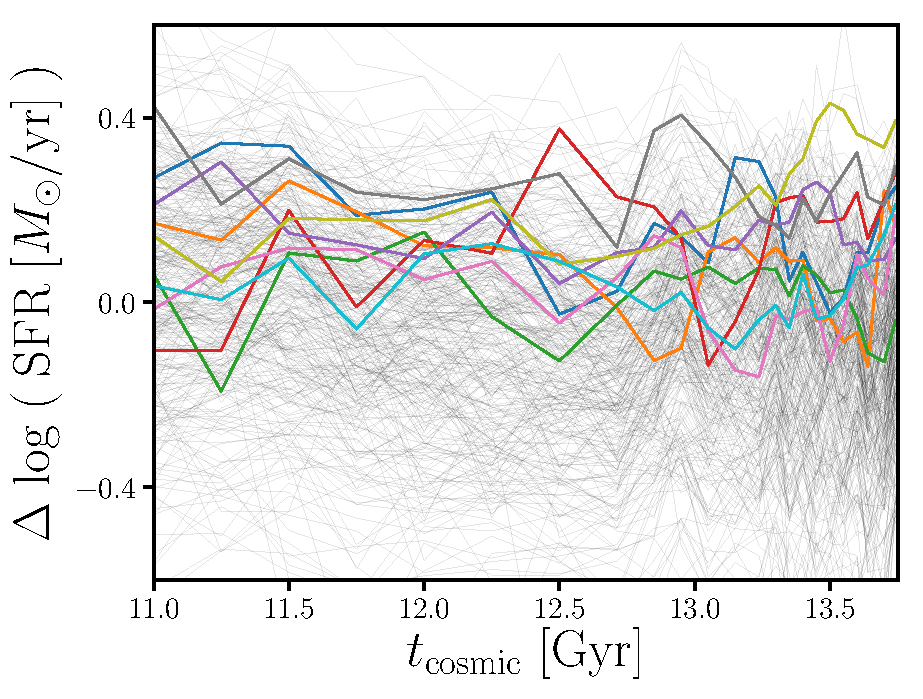
\includegraphics[width=0.5\textwidth]{figs/illustris_sfh.pdf}
    \caption{Galaxies in the Illustris simulation have SFHs that evolve along the
    SFS, with their SFRs stochastically fluctuating about the $\logsfr$ of the SFS.
    We highlight $\Delta \logsfr$, SFR with respect to $\logsfrsfs$ (Eq.~\ref{eq:logsfr_sf}),
    for a handful of galaxies with $10^{10.5}< M_* < 10^{10.6}M_\odot$ at $z\sim0$.
    We calculate $\Delta \logsfr$ with $\logsfrsfs$ identified using the \cite{hahn2018a}
    method, same as in Section~\ref{sec:sfcen}. The implementation of $\mathrm{SFR}$
    variability in the SFHs of star-forming centrals in our model (Section~\ref{sec:modelevol})
    is motivated by the SFHs of Illustris galaxies above.
    }
\label{fig:illsfh}
\end{center}
\end{figure}
%%%%%%%%%%%%%%%%%%%%%%%%%%%%%%%%%%%%%

%%%%%%%%%%%%%%%%%%%%%%%%%%%%%%%%%%%%%
% Figure 4
%%%%%%%%%%%%%%%%%%%%%%%%%%%%%%%%%%%%%
\begin{figure}
\begin{center}
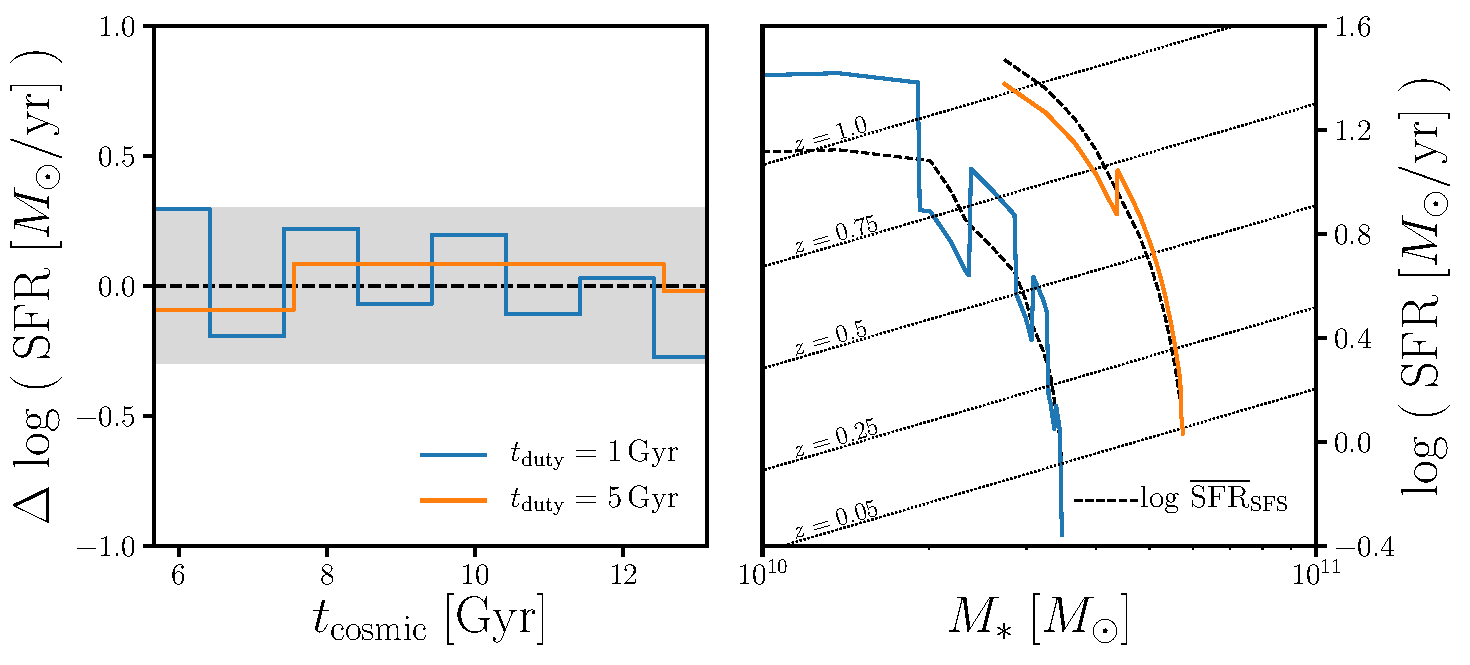
\includegraphics[width=0.85\textwidth]{figs/sfh_pedagogical.pdf}
    \caption{We incorporate star formation variability in our model using a
    ``star formation duty cycle'' where the SFRs of SF centrals fluctuate about
    the $\logsfrsfs$ on some timescale $t_\mathrm{duty}$. In our fiducial
    prescription, we randomly sample $\Delta \logsfr$ from a log-normal
    distribution with $0.3$ dex scatter at each timestep. We illustrate
    $\Delta\logsfr_i(t)$ of two SF centrals with star formation duty cycles
    on $t_\mathrm{duty} = 1$ Gyr (blue) and $5$ Gyr (orange) timescales
    in the left panel. $\Delta \logsfr(t)$ determines the SFH and hence
    the $M_*$ growth of the SF central galaxies (Eq.~\ref{eq:integ_mass}).
    On the right, we illustrate the $\mathrm{SFR}$ and $M_*$ evolutions
    of the corresponding SF centrals. For reference, we include
    $\logsfrsfs(M_{*,i}(t), t)$ that the galaxies' SFR and $M_*$ evolve along
    (black solid). We also include $\logsfrsfs(M_*)$ at various redshifts
    between $z = 1$ to $0.05$ (dotted  lines). \emph{The star-forming
    centrals in our model evolve their SFRs and $M_*$ along the SFS
    with their SFRs fluctuate about $\logsfrsfs$}.} \label{fig:sfh_model}
\end{center}
\end{figure}
%%%%%%%%%%%%%%%%%%%%%%%%%%%%%%%%%%%%%


\subsection{Evolving along the Star Formation Sequence} \label{sec:modelevol}
The tight correlation between the SFRs and stellar masses of star-forming
galaxies on the SFS has been observed spanning over four orders of magnitude
in stellar mass, with a roughly constant scatter of ${\sim}0.3$ dex, and out
to $z > 2$
(\emph{e.g.}~\citealt{noeske2007,daddi2007,elbaz2007,salim2007,santini2009,karim2011,whitaker2012,moustakas2013,lee2015}; see also references in \citealt{speagle2014}).
This correlation is also predicted by modern galaxy formation models~\citep[][see
\citealt{hahn2018a} and references therein]{somerville2015}. The SFS
naturally presents itself as an anchoring relationship to characterize
the star formation and $M_*$ growth histories of SF galaxies throughout $z < 1$. More
specifically, \emph{we characterize the SFH of each star-forming central
with respect to the $\logsfr$ of the SFS} (Eq.~\ref{eq:logsfr_ms}):
\beq \label{eq:logsfr_sf}
\logsfr_i(M_*, t) = \logsfrsfs(M_*, t) + \Delta\logsfr_i(t).
\eeq
Since SFHs determine the $M_*$ growth of galaxies, in this prescription,
$\Delta \logsfr_i(t)$ dictates the SFH and $M_*$ evolution of SF central.

One simple prescription for $\Delta \logsfr(t)$ would be to keep $\Delta \logsfr$
fixed throughout $z < 1$ to the offsets from the $\logsfrsfs$ in the
initial SFRs of our SF centrals at $z\sim1$ similar to simple analytic
models such as \cite{mitra2015}. Galaxies with higher than average
initial SFRs continue evolving above the average SFS, while SF centrals
with lower than average initial SFRs continue evolving below the average
SFS. In addition to not being able to reproduce observations, which we
later demonstrate, we also do not find such SFHs in SF galaxies of
hydrodynamic simulations such as Illustris~\citep{vogelsberger2014,genel2014}.
In Figure~\ref{fig:illsfh}, we plot $\Delta \logsfr_i$ of star-forming
galaxies in the Illustris simulation as a function of cosmic time. These
galaxies have stellar masses within $10^{10.5}-10^{10.6}M_\odot$ at $z=0$.
At each simulation output, we calculate $\Delta \logsfr_i$ using Eq.~\ref{eq:logsfr_sf}
with $\logsfrsfs$ derived from the SFS identified
\edt{in the simulation}
using the \cite{hahn2018a} method, same as in Section~\ref{sec:sfcen}. As the
highlighted $\Delta \logsfr_i$ illustrate, SF galaxies in Illustris evolve
along the SFS, with their SFRs fluctuating about $\logsfrsfs$.

Motivated by the SFHs of Illustris SF galaxies, we introduce variability
to the SFHs of our SF centrals in the form of a ``\emph{star formation duty cycle}''.
Within the Eq.~\ref{eq:logsfr_sf} SFH, we parameterize $\Delta \logsfr_i$ to
fluctuate about the $\logsfrsfs$ on timescale, $t_\mathrm{duty}$, with
amplitude sampled from a log-normal distribution with $0.3\,\mathrm{dex}$
scatter. For our fiducial star formation duty cycle prescription, we randomly
sample $\Delta \logsfr_i$ from a log-normal distribution with
\edt{$0.3\,\mathrm{dex}$ scatter}.
We illustrate $\Delta \logsfr_i(t)$ of SF centrals with our star formation
duty cycle prescription on $t_\mathrm{duty}=1$ Gyr (blue) and $5$ Gyr (orange)
timescales in the left panel of Figure~\ref{fig:sfh_model}.
The shaded region represents the observed $0.3\,\mathrm{dex}$ scatter of
$\logsfr$ in the SFS. This $\Delta \logsfr$ prescription by construction
reproduces the observed log-normal SFR distribution of the SFS
at any point in the model. Although, we do not expect this simplified
prescription to reflect the individual SFHs of SF centrals,
we seek to statistically capture the stochasticity from gas accretion,
star-bursts, and feedback mechanisms for the entire SF population.
Measuring $t_\mathrm{duty}$ in the duty cycle parameterization
provides us with an estimate of the timescale of such star formation
variabilities and thus provide additional useful constraints on the
physics of galaxy formation.

Using our fiducial SFH prescription, we evolve both the SFR and $M_*$
of our SF centrals along the SFS. Based on Eq.~\ref{eq:logsfr_sf},
the SFRs of our SF centrals are functions of $M_*$, while $M_*$
is the integral of the SFR over time:
\beq \label{eq:integ_mass}
M_*(t) = f_\mathrm{retain} \int\limits_{t_0}^{t} \mathrm{SFR(M_*, t')}\,\mathrm{d}t' + M_0.
\eeq
$t_0$ and $M_0$ are the initial cosmic time and stellar mass at $z \sim 1$,
respectively. $f_\mathrm{retain}$ here is the fraction of stellar mass
that is retained after supernovae and stellar winds; we use
$f_\mathrm{retain} = 0.6$~\citep{wetzel2013}. We can now evolve the SFR and
$M_*$ of our SF centrals until the final $z=0.05$ snapshot by
solving the differential equation of Eqs.~\ref{eq:logsfr_sf} and~\ref{eq:integ_mass}.
On the right panel of Figure~\ref{fig:sfh_model}, we present the
$\mathrm{SFR}$ and $M_*$ evolutions of two SF centrals with
$t_\mathrm{duty}=1$ Gyr (blue) and $5$ Gyr (orange), same
as the left panel. For reference, we include the mean $\logsfr$ of the SFS
that the galaxies' SFR and $M_*$ evolve along, $\logsfrsfs(M_{*,i}(t), t)$
(black solid). We also include $\logsfrsfs(M_*)$ (dotted lines) at various
redshifts between $z = 1$ to $0.05$. Based on the SFH prescription in our
model, SF centrals evolve their SFRs and $M_*$ along the SFS
with their SFRs fluctuate about $\logsfrsfs$.

%%%%%%%%%%%%%%%%%%%%%%%%%%%%%%%%%%%%%
% Figure
%%%%%%%%%%%%%%%%%%%%%%%%%%%%%%%%%%%%%
\begin{figure}
\begin{center}
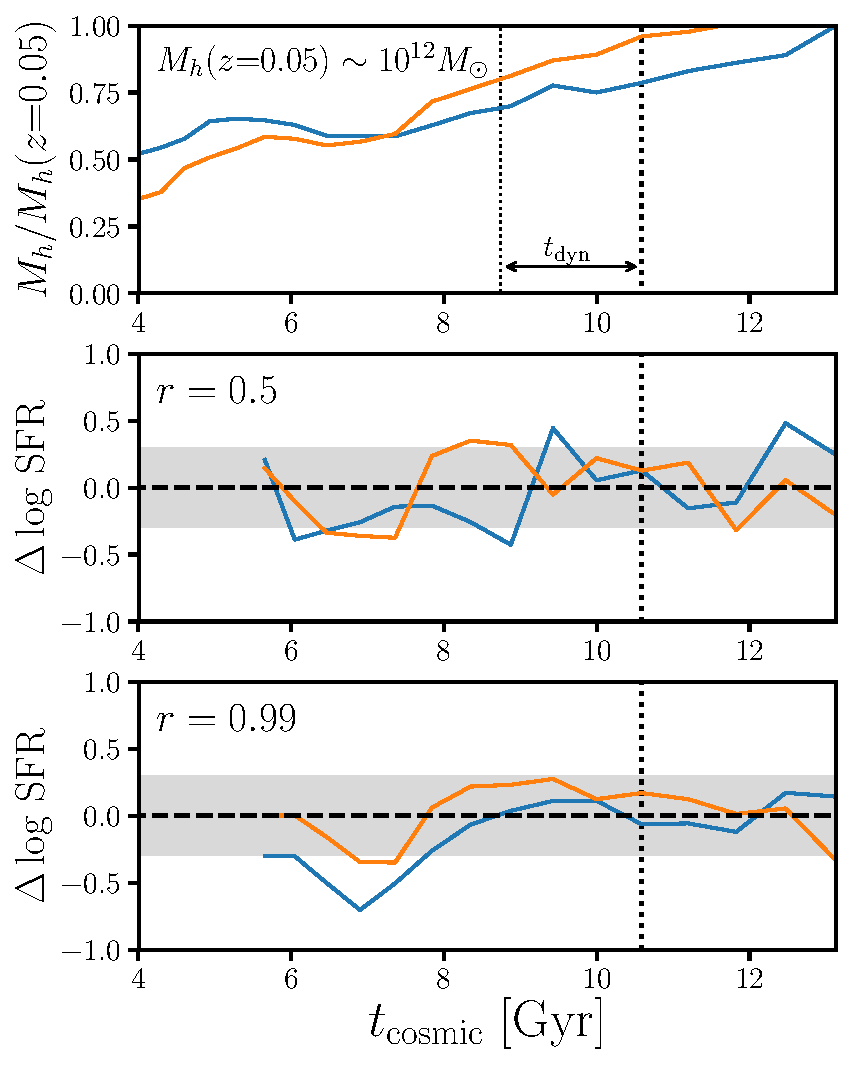
\includegraphics[width=0.5\textwidth]{figs/Mhacc_dSFR.pdf}
\caption{We incorporate assembly bias into the SF centrals of our model by
    correlating their host halo accretion history with their SFH with respect
    to the SFS. We plot the relative halo accretion history, $M_h(t)/M_h(z{=}0.05)$
    for two randomly chosen SF centrals with $M_h(z{=}0.05)\sim10^{12}M_\odot$,
    in the top panel. In the two panels below we present $\Delta\log\,\mathrm{SFR}$,
    SFH with respect to the SFS, of these galaxies for our model with correlation
    coefficients $r=0.5$ and $0.99$ (middle and bottom). The shaded region in these
    panels mark the $0.3$ dex 1-sigma width of the SFS. At some $t$ (dotted),
    $\Delta\log\,\mathrm{SFR}(t)$ is correlated with halo accretion over the
    period $t - t_\mathrm{dyn}$ to $t_\mathrm{dyn}$ labeled in top panel. The
    SFHs illustrate how $\Delta\log\,\mathrm{SFR}(t)$ correlates with
    $\Delta M_h = M_h(t) - M_h(t-t_\mathrm{dyn})$ and how $\Delta\logsfr(t)$
    correlates more strongly with $\Delta M_h(t)$ with higher $r$.}
\label{fig:mhacc_dsfr}
\end{center}
\end{figure}
%%%%%%%%%%%%%%%%%%%%%%%%%%%%%%%%%%%%%
\subsection{Adding Assembly Bias}
\edt{In our fiducial SFH precription, we sample $\Delta \logsfr_i$ randomly
from a log-normal distribution with $0.3$dex scatter.}
There is, however, growing evidence that star formation in galaxies correlate with their host
halo accretion histories~\citep[\emph{e.g.}][]{lim2016, tojeiro2017, tinker2018b}.
Therefore, in this section, we describe how we introduce \emph{assembly bias}
into the SFH prescription of our model.% and investigate its impact on $\sigma_{\log M_*}$.
Assembly bias, most commonly in the literature, refers to the dependence of the
spatial distribution of dark matter halos on halo properties besides
mass~\citep{gao2005,wechsler2006,gao2007,wetzel2007,li2008,sunayama2016}.
At low halo mass, older and more concentrated halos form in high density environments.
While at high halo mass, the effect is the opposite --- younger, less concentrated
halos form in high-density regions. However, both
simulations~\citep{croton2007, artale2018, zehavi2018} as well as
observations~\citep{yang2006,wang2008,tinker2011,wang2013,lacerna2014,calderon2018,tinker2018},
\ch{@JLT I'm not sure which citations you're referring to.}
find that this assembly bias propagates beyond spatial clustering and correlates
with \edt{certain} galaxy properties such as formation histories and star formation
properties, an effect more specifically referred to as {\em galaxy} assembly bias.
In our model, we incorporate galaxy assembly bias by correlating the SFHs
of our SF central galaxies and their host halo accretion histories
with a correlation coefficient $r$.

We correlate a galaxy's SFR with respect to the mean SFS SFR
(\emph{i.e.} $\Delta\log\,\mathrm{SFR}$ in Eq.~\ref{eq:logsfr_sf}) to the
halo mass accretion over dynamical time. At every $t_\mathrm{duty}$ timestep,
$t$, $\Delta\logsfr(t)$ is assigned based on
$\Delta M_h(t) = M_h(t) - M_h(t - t_\mathrm{dyn})$ in $M_\mathrm{max}$ bins
with a correlation coefficient $r$, a parameter added to our model. This
prescription for correlating $\Delta\log\,\mathrm{SFR}$ to $\Delta M_h$ is
similar to other empirical models that also correlate $\Delta\log\,\mathrm{SFR}$
to $\Delta M_h$ over $t_\mathrm{dyn}$~\citep{rodriguez-puebla2016a, behroozi2018}.
In \cite{rodriguez-puebla2016a}, however, they assume perfect ($r=1$) correlation
between SFH and halo accretion. In the \cite{behroozi2018} {\sc UniverseMachine}
(hereafter UM), $r$ is free parameter and their SFH includes SF variability,
similar to our model. As we mention in the introduction, their prescription,
however, does not not focus on a star formation variation on specific timescales as our model does through
the star formation duty cycle.

In Figure~\ref{fig:mhacc_dsfr} we illustrate this prescription for galaxy
assembly bias in our model. We plot the relative halo accretion histories
$M_h(t)/M_h(z{=}0.05)$ of two arbitrarily chosen SF centrals with
$M_h(z{=}0.05)\sim10^{12}M_\odot$ in the top panel (orange and blue). Below, we plot
$\Delta\logsfr$, SFH with respect to the SFS, of these galaxies for our model with
correlation coefficients $r=0.5$ and $0.99$ (middle and bottom). We choose a
random $\mathtt{TreePM}$ snapshot, $t$ (dotted), and label the period
[$t$, $t - t_\mathrm{dyn}$]. Halo accretion over this period,
$\Delta M_h = M_h(t) - M_h(t-t_\mathrm{dyn})$, correlates with $\Delta\logsfr(t)$.
The SFHs in the middle and bottom panels illustrate this correlation and how
$\Delta\logsfr(t)$ correlates more strongly with $\Delta M_h(t)$ for our model
with higher $r$.

\subsection{\edt{$\sigma_{\log\,M_*}$ at $z=1$}}
\edt{So far in both our fiducial and assembly bias added models above, we make the
assumption that the log-normal scatter in $M_*$ at fixed $M_h$ at $z\sim1$,
$\sigma_{\log\,M_*}(M_h; z=1) = 0.2$ dex. This initial condition determines
the initial SHAM $M_*$ at $z\sim1$ that initializes our models and is motivated
by constraints on the observed
SHMR~\citep[\emph{e.g.}][]{leauthaud2012, tinker2013, patel2015}. However,
these $\sigma_{\log\,M_*}(M_h; z=1)$ constraints are derived using halo models
in which $\sigma_{\log\,M_*}(z = 1)$ is a constant, independent of $M_h$.
For these models, the constraining power mainly come from massive halos.
Hence, the $0.2$ dex constraint does not accurately reflect $\sigma_{\log\,M_*}(z\sim1)$
for less massive halos ($M_h < 10^{12}M_\odot$).
Later in this paper we focus on $\sigma_{\log\,M_*}(M_h=10^{12}M_\odot; z=0)$
predicted by our models. We therefore examine the impact of varying
$\sigma_{\log\,M_*}(z\sim1)$ on $\sigma_{\log\,M_*}(M_h=10^{12}M_\odot; z=0)$
by introducing models with $\sigma_{\log\,M_*}(M_h; z=1) = 0.35$ and 0.45 dex.
Our choice is based on the $z=1$ SHMR in the Illustris TNG~\citep{pillepich2018}
cosmological hydrodynamic simulation, which has $\sigma_{\log\,M_*}(z\sim1)$
spanning $0.4$ to $0.2$ dex for $M_h = 10^{10.5}M_\odot$ to $10^{11.5}M_\odot$.}

\edt{All of the models we present in this section track the SFRs and $M_*$ of SF
central galaxies. We can compare these properties of our model galaxies
to observed galaxy population statistics (quiescent fraction and SMF) to
constrain the model free parameters.}
Our models, run with these inferred
parameters, can then be compared to observations of the galaxy-halo connection
such as the SHMR. In the following section, we present this comparison and
the constraints we derive on the role and timescale of star formation
variability in SF central galaxies.

%%%%%%%%%%%%%%%%%%%%%%%%%%%%%%%%%%%%%
% Figure 4
%%%%%%%%%%%%%%%%%%%%%%%%%%%%%%%%%%%%%
\begin{figure}
\begin{center}
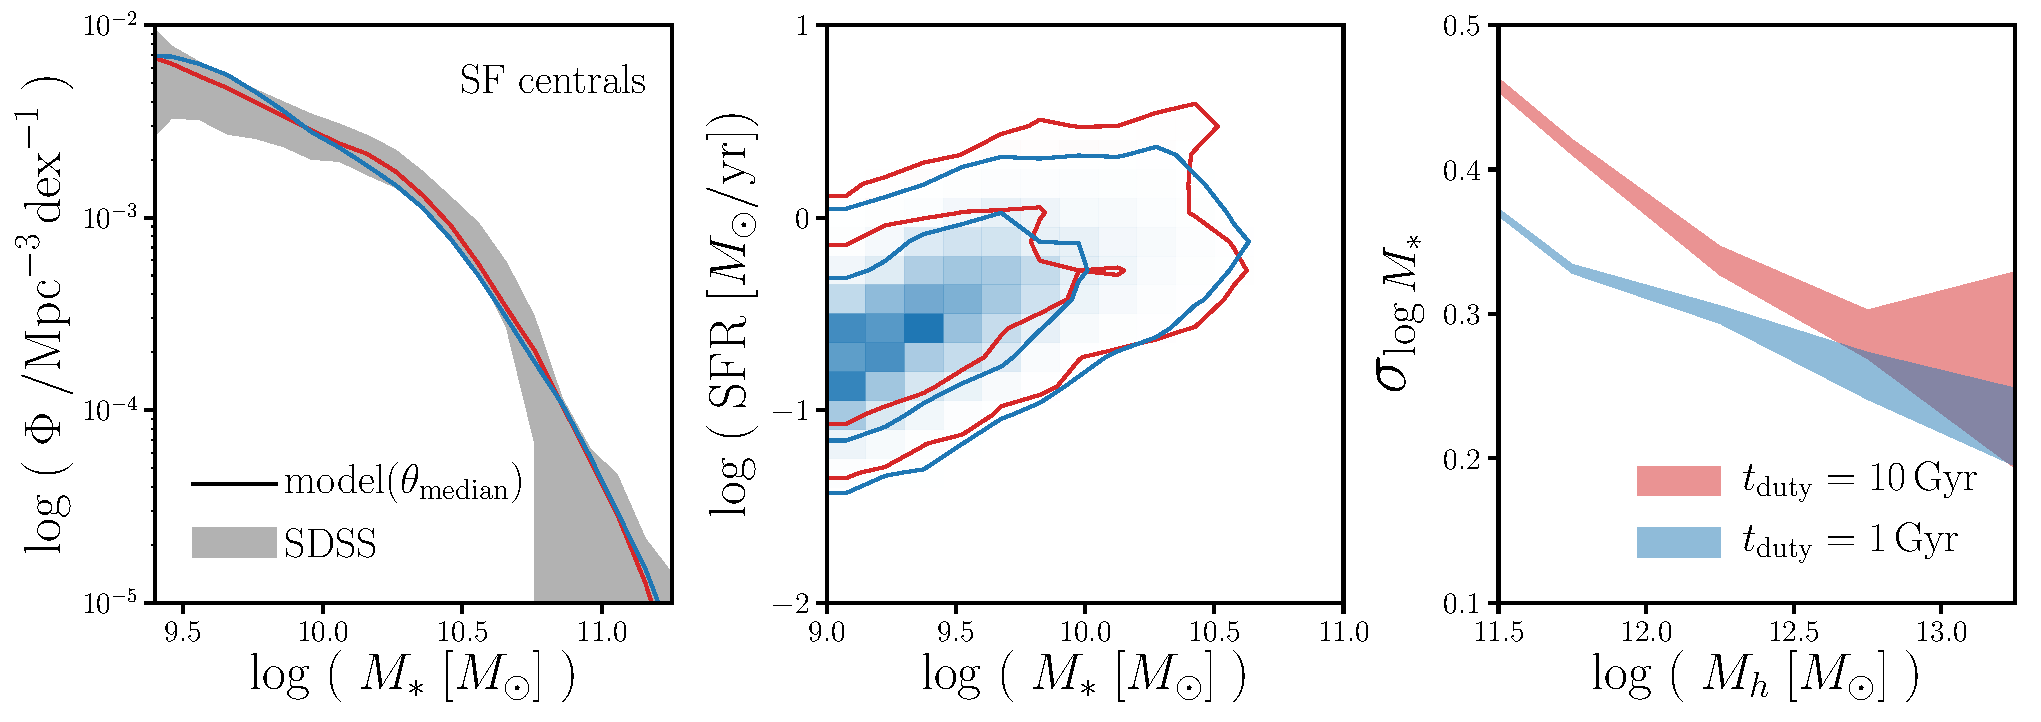
\includegraphics[width=\textwidth]{figs/qaplot_abc.pdf}
    \caption{Our models with different star formation duty cycle timescales
    (blue: $t_\mathrm{duty}{=}1\,\mathrm{Gyr}$; red: $t_\mathrm{duty}{=}10\,\mathrm{Gyr}$)
    run with median values of their ABC posterior distribution have SMFs and SFSs consistent
    with observations (left and middle). \emph{They however produce significantly different
    scatter in $\log\,M_*$ at fixed $\log\,M_\mathrm{halo}$ --- scatter in the SHMR (right)}.
    By comparing the scatter in SHMR of our models to observational constraints on the SHMR,
    we constrain the timescale of the star formation duty cycle and thereby the SFHs of star
    forming galaxies.
    }
\label{fig:abc_demo}
\end{center}
\end{figure}
%%%%%%%%%%%%%%%%%%%%%%%%%%%%%%%%%%%%%

\section{Results and Discussion} \label{sec:results}
Our models take $\mathtt{TreePM}$ central subhalos and tracks their SFR
and $M_*$ evolution using flexible parameterizations of the SFS and SFHs
that incorporate variability through a star formation duty cycle.
At $z = 0.05$, the final timestep, our models predict SFR and $M_*$ of SF
centrals, along with their host halo properties. We now use these resulting
properties to compare our model to observations and constrain its free
parameters --- the SFS parameters of Eq.~\ref{eq:logsfr_ms}. Since we focus
on SF centrals, the main observable we use is the SMF of SF centrals in
SDSS, which we estimate as
\beq \label{eq:smf_sf_cen}
\Phi^\mathrm{SDSS}_\mathrm{SF,cen} = f^\mathrm{cen}_\mathrm{SFS} \times f_\mathrm{cen} \times \Phi^\mathrm{Li\&White(2009)}.
\eeq
$f^\mathrm{cen}_\mathrm{SFS}$ is the fraction of central galaxies on the
SFS, which we fit in Eq.~\ref{eq:f_cen_sfms}. $f_\mathrm{cen}$ is the
central galaxy fraction from \cite{wetzel2013} and $\Phi^\mathrm{Li\&White(2009)}$
is the SMF of the SDSS from \cite{li2009}. If our models reproduce the
observed $\Phi^\mathrm{SDSS}_\mathrm{SF,cen}$, by construction they reproduce
the observed quiescent fraction.

For the comparison between our models and observation, we use the likelihood-free parameter
inference framework of Approximate Bayesian Computation (ABC). ABC has the
advantage over standard approaches to parameter inference in that it does not
require evaluating the likelihood. For observables with likelihoods that are
difficult or intractable, incorrect assumptions in the likelihood can significantly
bias the posterior distributions~\citep[\emph{e.g.}][]{hahn2018}. Instead,
ABC relies only on a simulation of the observed data and a distance metric to
quantify the ``closeness'' between the observed data and simulation. Many variations
of ABC has been used in astronomy and
cosmology~\citep[\emph{e.g.}][]{cameron2012,weyant2013,ishida2015,alsing2018}.
We use ABC in conjunction with the efficient Population Monte Carlo (PMC)
importance sampling as in~\citep{hahn2017b, hahn2017a}. For initial sampling
of our ABC particles, \emph{i.e.} the priors of our free parameters
$m^\mathrm{low}_{M_*}$, $m^\mathrm{high}_{M_*}$, and $m_z$, we use uniform
distributions over the ranges $[0.0, 0.8]$, $[0.0, 0.8]$, and
$[0.5, 2.]$, respectively. The range of the prior were conservatively chosen
to encompass the best-fit SFS from~\cite{speagle2014}
and measurements from~\cite{moustakas2013} and~\cite{lee2015} at $z \sim 1$.
Finally, for our distance metric we use the following distance between
the SMF of the star-forming centrals in our model to the observed
$\Phi^\mathrm{SDSS}_\mathrm{SF,cen}$:
\beq
\rho_\Phi = \sum\limits_{M} \left( \frac{\Phi^\mathrm{sim} - \Phi^\mathrm{SDSS}_\mathrm{SF,cen}}{\sigma'_\Phi}\right)^2.
\eeq
$\Phi^\mathrm{sim}(M)$ above is the SMF of the SF centrals in our model
and $\sigma'_\Phi(M)$ is the uncertainty of $\Phi^\mathrm{SDSS}_\mathrm{SF,cen}$,
which we derive by scaling the~\cite{li2009} uncertainty of $\Phi^\mathrm{SDSS}$
derived from mock catalogs. %\todo{We emphasize that ABC is not very sensitive to the distance metric.}
For the rest of our ABC-PMC implementation, we strictly follow the implementation
of~\cite{hahn2017a} and \cite{hahn2017b}. We refer reader to those papers for
further details.

%%%%%%%%%%%%%%%%%%%%%%%%%%%%%%%%%%%%%
% Figure 5
%%%%%%%%%%%%%%%%%%%%%%%%%%%%%%%%%%%%%
\begin{figure}
\begin{center}
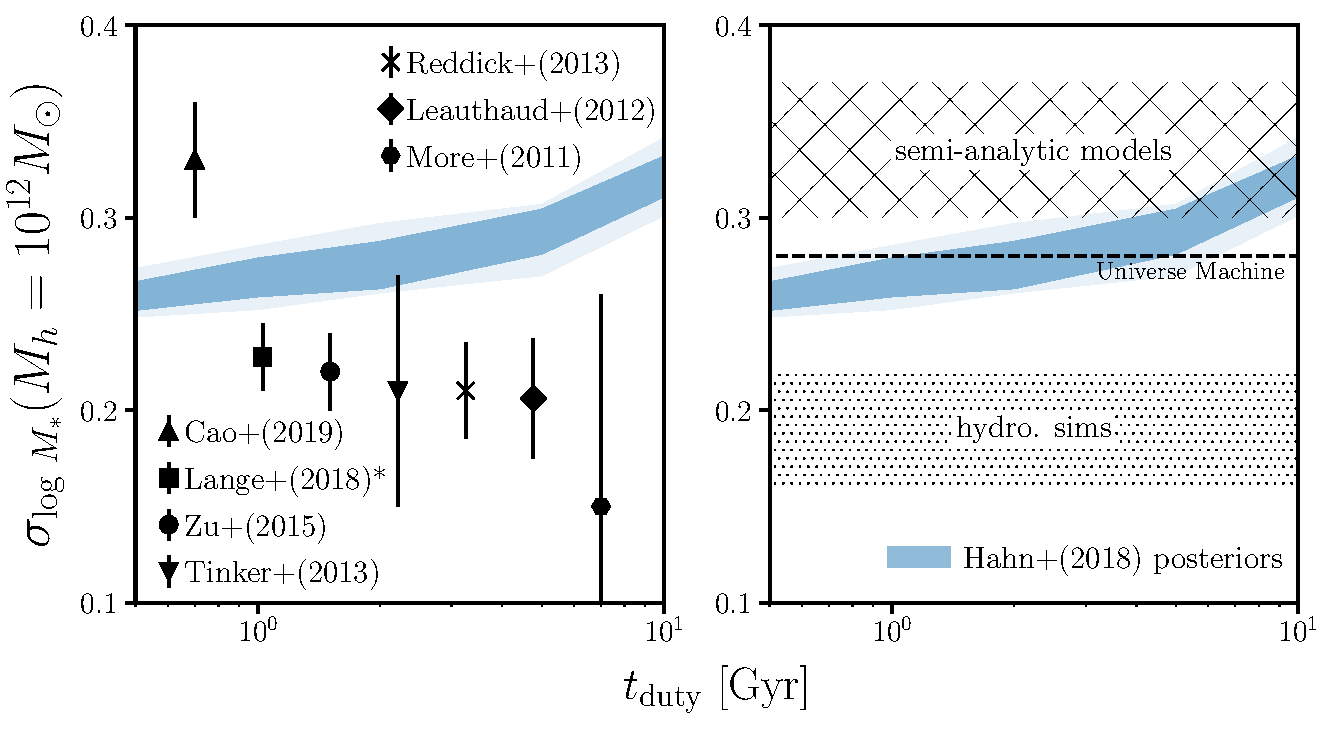
\includegraphics[width=0.75\textwidth]{figs/SHMRscatter_tduty_v2.pdf}
    \caption{With shorter star formation duty cycle timescales, $t_\mathrm{duty}$,
    our \edt{fiducial}
    model predicts smaller scatter in $\log M_*$ at
    $M_h = 10^{12} M_\odot$ --- $\sigma_{\log\,M_*}$ (blue). The dark and light blue
    shaded regions represent the $68\%$ and $95\%$ confidence
    intervals of $\sigma_{\log\,M_*}$ predicted from the ABC posteriors of our
    model with $t_\mathrm{duty} = 0.5, 1, 2, 5$, and $10$ Gyr. For $t_\mathrm{duty} = 10$
    to $0.5\,\mathrm{Gyr}$, $\siglogm$ ranges from $0.32\substack{+0.02\\ -0.02}$ to
    $0.26\substack{+0.01\\-0.01}$. In the left panel, we include for comparison
    observational $\siglogm$ constraints from \cite{yang2009, more2011, leauthaud2012, zu2015, tinker2017, lange2018a}
    and Cao et al. (in preparation), described in Section~\ref{sec:sfdutycycle}.
    %\edt{\cite{lange2018a} constrains the scatter in $\log L$ at $M_h = 10^{12} M_\odot$}.  \edt{$\sigma_{\log\,M_*}$ constraints from the literature, besides Cao et al. (in preparation),  are derived using halo models where the constraining power mainly come from massive halos.}
    In the right panel, we include compiled predictions from hydrodyanmic simulations
    (dotted region), semi-analytic models (hatched), and
    \edt{the~\cite{behroozi2018} {\sc UM} empirical model. We also include $\siglogm$
    from a simple empirical model with \cite{abramson2016} SFHs assigned to halos via
    abundance matching (dotted).}
    \edt{\emph{A shorter $\tduty$ produces significantly tighter scatter in the SHMR.
    Observational constraints and predictions from hydrodynamic simulations
    favor a star formation variability on $\tduty \lesssim 1$ Gyr for our fiducial
    model.}}
    }
\label{fig:sigMstar_duty}
\end{center}
\end{figure}
%%%%%%%%%%%%%%%%%%%%%%%%%%%%%%%%%%%%%

%\subsection{Timescale of the Star Formation Duty Cycle} \label{sec:sfdutycycle}
\subsection{\edt{The Fiducial Model}} \label{sec:sfdutycycle}
We present the SMFs (left), SFSs (center), and the scatter in $\log M_*$ at $M_h$,
$\sigma_{\log\,M_*}(M_h)$, (right) of our
\edt{fiducial}
model run using SFHs with two different duty cycle timescales, $t_\mathrm{duty} = 10$ (red)
and $1\,\mathrm{Gyr}$ (blue), in Figure~\ref{fig:abc_demo}. For each $\tduty$,
we evaluate our fiducial model at the median parameter values of the respective
posterior distributions derived using ABC. For both $\tduty$, our model
successfully produces SMFs, $\Phi^{\rm SDSS}_{\rm SF,cen}$, and SFSs consistent
with observations, as expected (left and center panels). Despite their consistency
with observations, however, different $t_{\rm duty}$ of the models predict i
significantly different $\sigma_{\log\,M_*}$, particularly below $M_h < 10^{12.5}M_\odot$.
We further illustrate the sensitivity of $\sigma_{\log\,M_*}$ of our model to
$\tduty$ in Figure~\ref{fig:sigMstar_duty}, where we present $\sigma_{\log\,M_*}$ at
fixed halo mass $M_h = 10^{12} M_\odot$ for our model with $t_{\rm duty} = 0.5, 1, 2, 5$,
and $10$ Gyr. As in Figure~\ref{fig:abc_demo}, $\sigma_{\log\,M_*}$ at each $t_{\rm duty}$
is predicted from our model with parameters from the corresponding ABC posterior
distribution. The dark and light blue shaded regions represents the $68\%$ and $95\%$
confidence intervals. For $t_\mathrm{duty}$ ranging from $10$ to $0.5\,\mathrm{Gyr}$,
$\sigma_{\log\,M_*}$ ranges from
$0.32\substack{+0.02\\ -0.02}$ to $0.26\substack{+0.01\\-0.01}$
--- a shorter star formation duty cycle timescale produces significantly
smaller scatter in the SHMR. \emph{Observational constraints on the SHMR
can therefore be used to constrain the timescale of star formation
variability and SFH of SF central galaxies.}

On the left panel of Figure~\ref{fig:sigMstar_duty}, we compare
$\sigma_{\log M_*}$ predicted from our fiducial model to observational
constraints in the literature. These constraints are mainly derived from
fitting halo-occupation based models to observations of galaxy
clustering, SMF, satellite kinematics, or galaxy-galaxy weak lensing. In
Figure~\ref{fig:sigMstar_duty}, we include $\sigma_{\log M_*}$ constraints
from~\cite{more2011, leauthaud2012, reddick2013, tinker2013, zu2015} and
Cao et al. (in preparation). \cite{more2011}, \cite{reddick2013}, and \cite{zu2015}
fit SDSS DR7 measurements of satellite kinematics, projected galaxy clustering and
conditional SMF, and, galaxy clustering and galaxy-galaxy
lensing, repsectively. Meanwhile, \cite{leauthaud2012, tinker2013}
use COSMOS to fit the SMF, galaxy clustering, and galaxy-galaxy lensing.
Finally, Cao et al. (in preparation) fit the kurtosis of the line-of-sight
pairwise velocity dispersion between central galaxies and all neighboring
galaxies to constrain the scatter in SHMR at low halo masses. We note that
\cite{leauthaud2012, reddick2013, zu2015} measure $\sigma_{\log M_*}$ for
all central galaxies, not only SF. Both \cite{more2011, tinker2013},
however, find a $< 1\sigma$ difference in $\sigma_{\log M_*}$ between SF
and quiescent centrals, so we include these constraints in our comparison.
We also include the \cite{lange2018a} constraint from fitting color-dependent
conditional luminosity function and radial profile of satellite galaxies
of SDSS DR7. We note that this constraint is on the scatter in luminosity,
$\log L$, not $\log M_*$ at a given $M_h$.

%We find that by decreasing the timescale of stochasticity on a simple SFH model that traces the overall
%SFS evolution does in fact decrease the scatter seen in the SMHMR.
%The $\sigma_{\log\,M_h}$ constraints from the literature are significantly scatter from $0.12$ to $0.6\,\mathrm{dex}$, right panel of Figure~\ref{fig:sigMstar_duty}.  $\sigma_{\log\,M_h}$ from our model, regardless of $t_\mathrm{duty}$ is well within this range, so the comparison does not provide much constraint on $t_\mathrm{duty}$. On the other hand,
\edt{Besides Cao et al. (in preparation), the $\sigma_{\log\,M_*}$ constraints
in the literature are loosely consistent with $\sigma_{\log\,M_*} \sim 0.2$ dex.
These constraints, however, are mostly derived using halo models that assume
$\sigma_{\log\,M_*}$ is constant independent of $M_h$. The constraining power for
these constraints mainly come from high mass halos and, thus, do not reflect
$\sigma_{\log\,M_*}$ at $M_h=10^{12}M_\odot$}.
While \cite{reddick2013} constrain $\sigma_{\log\,M_*}$ for different bins of
$M_h$ over the range $10^{12} - 10^{14} M_\odot$, %and find little $M_h$ dependence in $\sigma_{\log\,M_*}$,
their constraints mainly come from the conditional SMF and therefore relies on
the accuracy of the \cite{tinker2011} group finder in identifying halo masses.
\ch{JLT: Why does Reddick come from $10^{13} M_\odot$?} %Group finder based halo masses can over- or under-estiamte halo masses by an order of magnitude~\citep{old2014}.
The constraint from \cite{lange2018a} is also derived from a halo model
with $M_h$ dependence. However, as mentioned above, they constrain $\sigma_{\log\,L}$.
In \cite{more2011}, where they constrain both $\sigma_{\log\,L}$ and $\sigma_{\log\,M_*}$
from the same data, they find
$\sigma_{\log\,M_*} = 0.15\substack{+0.08\\ -0.11} < \sigma_{\log\,L} = 0.21\substack{+0.06\\ -0.04}$
for blue centrals. However, translating from $\sigma_{\log\,L}$ to
$\sigma_{\log\,M_*}$ is tenuous for different data sets and models. %Overlooking the varoius caveats of the analyses, $\sigma_{\log\,M_*}$ from Cao et al. (in preparation) is in tension with the other constraints.  \ch{JLT: sentence on the Cao et al. discrepancy?}.
\edt{We also note observational constraints include significant measurement
uncertainties in $M_*$. The intrinsic $\sigma_{\log\,M_*}$ of these constraints,
\emph{i.e.} the scatter predicted by our model, will be lower. If we consider
$0.1 - 0.2$ dex uncertainties in $M_*$~\citep{roediger2015}, the
Cao et al. (in preparation) constraint, for instance, will be reduced from
$\sigma_{\log\,M_*} = 0.33$ dex to $0.31 - 0.26$ dex. Overall, observational
constraints favor a shorter, $< 2$ Gyr, duty cycle timescale for our fiducial
model.}

In addition to the observational constraints, we also compare the $\sigma_{\log\,M_*}(M_h \sim 10^{12}M_\odot)$
predicted by our model to predictions from modern galaxy formation models
on the right panel: hydrodynamic simulations (dot filled), semi-analytic models
(SAM; hatched), and an empirical model (dashed line). For the hydrodynamic simulations,
the dotted region, $\sigma_{\log\,M_*} = 0.16 - 0.22$ dex, encompasses
predictions from EAGLE~\citep{matthee2017}, Massive Black II~\citep{khandai2015},
and Illustris TNG, as compiled in Figure 8 of \cite{wechsler2018}.
For the SAMs, the hatched region, $\sigma_{\log\,M_*} = 0.3 - 0.37$ dex,
includes predictions from~\cite{lu2014, somerville2012}, and the SAGE\footnote{\url{https://tao.asvo.org.au/tao/}}
model~\edt{\citep{croton2016}}. We also include the prediction from the
\cite{behroozi2018} UM empirical model. $\sigma_{\log\,M_*}$ from SAMs are
consistent with our model with $t_{\rm duty} \gtrsim 5$ Gyr. UM, which predicts
a lower $\sigma_{\log\,M_*}$, is consistent with $t_{\rm duty} = 1 - 5$ Gyr.
Lastly, hydrodynamic simulations predict the lowest $\sigma_{\log\,M_*}$ among
the models
\edt{with $\sim 0.2$ dex, which our fiducial model struggles to reproduce
even with the shortest $t_{\rm duty}$ timescale that we consider.
There is no consensus among the observational $\sigma_{\log\,M_*}$ constraints
at $M_h \sim 10^{12} M_\odot$. However, at $M_h > 10^{12} M_\odot$ observations
are in better agreement and {\em only} hydrodynamic simulations predict $\sigma_{\log\,M_*}$
low enough to be consistent~\citep{wechsler2018}. To reproduce observational
constraints and predictions from hydrodynamic simulations, SF central galaxies
in our fiducial model require star formation varability on short timescales,
$\lesssim 1$ Gyr.}

A key element of our models is the SFH prescription for SF central galaxies where
the SFH evolves about the SFS. Contrary to our SFH prescription, \cite{kelson2014},
for example, argue that the SFS is a consequence of central limit theorem
and can be reproduced even if \emph{in situ} stellar mass growth is modeled as
a stochastic process like a random walk. \cite{gladders2013,abramson2015,abramson2016},
similarly argue that $\sim2000$ loosely constrained log-normal SFHs can reproduce
observations such as the SMF at $z \leq 8$ and the SFS at $z \leq 6$. These works,
however, focus on reproducing observations of galaxy properties and do not examine
the galaxy-halo connection such as the SHMR. In order to test whether log-normal
SFHs can also produce realistic SHMRs,
\edt{we construct a simple empirical model using  the SFHs, $\mathrm{SFR}(t)$ and
$M_*(t)$, from \cite{abramson2016} and assign them to halos by abundance matching
their $M_*$ to $M_h$ at $z{\sim}1$.}
We then restrict the SFHs to those that would be classified as star-forming based
on a $\log\,\mathrm{SSFR} > -11.$ cut. Afterwards we measure $\sigma_{\log\,M_*}$
at the lowest $M_h$ where it can be reliably measured given the \cite{abramson2016}
sample's $M_*{>}10^{10}M_\odot$ limit.
\edt{We find that the \cite{abramson2016} based empirical model predicts a scatter
of $\sigma_{\log\,M_*}(M_h=10^{12.4}) = 0.33\pm0.04$ (dotted; right panel of Figure~\ref{fig:sigMstar_duty}).
Although the \cite{abramson2016} SFHs can reproduce a number of galaxy observations,
without star formation varability on short timescales the empirical model struggles
to produce $\sigma_{\log\,M_*}$ comparable to observational constraints and predictions
from UM and hydrodynamic simulations.}

\edt{The \cite{abramson2016} based empirical model that we explore utilizes a simple
abundance matching scheme. \cite{diemer2017} find that their their log-normal fits
to the SFHs of Illustris galaxies correlate with halo formation histories. Incorporating
such correlations into the abundance matching may reduce $\sigma_{\log\,M_*}$.
In fact, although we demonstrate in this section that star formation variability
in the SFH on short timescales significantly reduces $\sigma_{\log\,M_*}(M_h=10^{12})$,
this alone is insufficient to produce the tight scatter in SHMR found in
observations and hydrodynamic simulations. In the next section, we explore how
correlation between SFH and halo formation histories impacts $\sigma_{\log\,M_*}(M_h=10^{12})$
using our models with assembly bias.
}
%All considered, despite the overall tension, {\em the observational constraints of $\sigma_{\log\,M_*}$ favor our model with a shorter duty cycle timescale.} %\emph{A short duty cycle timescale--- $t_\mathrm{duty} \lesssim 0.5\,\mathrm{Gyr}$--- is necessary for our model to ameliorate the tension with $\sigma_{\log\,M_*}$ constraints in the literature}.
%This $t_\mathrm{duty}$ constraint implies that SF galaxies have star formation variations on short timescales.
%However, even with the shortest duty cycle timescale we probe  {\color{red} ($\sigma_{\log\,M_*}{=}\,0.26\substack{+0.010\\ -0.012}$) } our model predicts $\sigma_{\log M_*}$ larger than in observations.

%%%%%%%%%%%%%%%%%%%%%%%%%%%%%%%%%%%%%
% Figure
%%%%%%%%%%%%%%%%%%%%%%%%%%%%%%%%%%%%%
\begin{figure}
\begin{center}
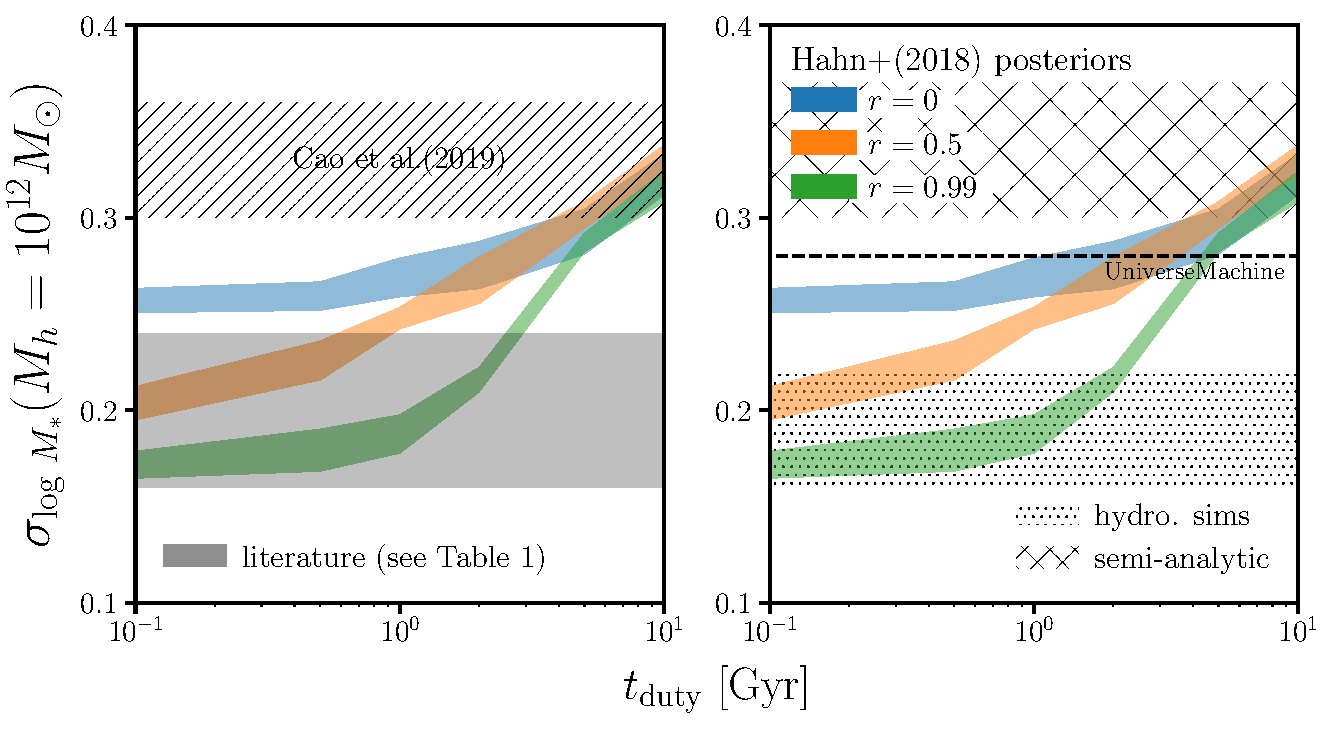
\includegraphics[width=0.75\textwidth]{figs/SHMRscatter_tduty_abias2.pdf}
    \caption{\edt{Our models that correlate SFH with halo assembly history ($r > 0$),
    predict $\siglogm$ that span the various observational constraints and predictions 
    from galaxy formation models.}
    We plot $\siglogm(M_h=10^{12}M_\odot)$ as a function of the star formation
    duty cycle timescale, $t_\mathrm{duty}$, for our
    \edt{models with $r = 0$ (no assembly bias; blue), 0.5 (orange), and 0.99 (green).
    We include observational cosntraints and predictions from galaxy formation models
    in the left and right panels.
    \emph{Stronger assembly bias significantly reduces the scatter in SHMR for
    $t_\mathrm{duty} < 5$ Gyr.}
    With our models with $r > 0.$ and $t_\mathrm{duty} < 2$ Gyr
    we can produce the tight scatter in SHMR ($\siglogm \sim 0.2$ dex) found in
    some of the observational cosntraints and predicted by hydrodynamic simulations}.
    }
\label{fig:sigMstar_duty_abias}
\end{center}
\end{figure}
%%%%%%%%%%%%%%%%%%%%%%%%%%%%%%%%%%%%%

\subsection{\edt{Models with Assembly Bias: $r > 0$}}
A shorter star formation duty cycle timescale produces tighter scatter in the
SHMR of our \edt{fiducial} model. This dependence on the duty cycle timescale,
allows us to compare the model with measurements of $\sigma_{\log M_*}$ and
predictions from galaxy formation models to constrain $t_\mathrm{duty}$, which
reflect the star formation variability timescale. Such comparisons in the previous
section, demonstrate that $t_\mathrm{duty} \lesssim 2\,\mathrm{Gyr}$ is
favored by observational constraints. However, a short duty cycle
timescale alone is not enough to conservatively reproduce the $\sigma_{\log\,M_*}$
\edt{constraints from some obsevations and predicted by hydrodynamic simulations.
Therefore, in this section, we examine how assembly bias impacts $\sigma_{\log M_*}$
using our models that correlate SFH with host halo accretion history ($r > 0$).}

We repeat our analysis of inferring model parameters by comparing to observations
using ABC-PMC --- this time for our model with galaxy assembly bias over a grid of
$t_{\rm duty}$ and $r$ values. Using the resulting posterior distributions, we
examine the scatter in the SHMR ($\sigma_{\log\,M_*}$) predicted by our model as a
function of $t_{\rm duty}$ with $r=0$ (no assembly bias; blue), $0.5$ (orange),
and $0.99$ (green) in Figure~\ref{fig:sigMstar_duty_abias}. The shaded regions
represent the $68\%$ confidence interval of the predicted $\sigma_{\log\,M_*}$.
We again emphasize that for all sets of ($t_{\rm duty}$, $r$) our models reproduce
the observed SMF of SF centrals and SFS.  At $t_\mathrm{duty} \geq 5\,\mathrm{Gyr}$
we find no significant difference in $\sigma_{\log\,M_*}$, regardless of $r$.
Below $t_\mathrm{duty} < 5\,\mathrm{Gyr}$, however, $\sigma_{\log\,M_*}$ of our
model decreases significantly as the SFH of SF galaxies are more correlated
with halo accretion history.  For $t_\mathrm{duty} = 0.5\,\mathrm{Gyr}$, we find
$\sigma_{\log\,M_*}{=}\,0.26\substack{+0.01\\-0.01},
0.22\substack{+0.01\\-0.01}$, and $0.17\substack{+0.01\\-0.02} $
for $r = 0.0, 0.5$, and $0.99$, respectively.

\edt{Comparing our $r > 0$ models to the observational constraints in
Figure~\ref{fig:sigMstar_duty}, we find that assembly bias significantly
reduces the tensions with observations (left panel of
Figure~\ref{fig:sigMstar_duty_abias})}.
With a short star formation duty cycle ($t_\mathrm{duty} \leq 1\,\mathrm{Gyr}$)
and galaxy assembly bias with $r \ge 0.5$, our model is in agreement with
these $\sigma_{\log\,M_*} \sim 0.2$ dex constraints. On the other hand,
assembly bias increases the tension with
\edt{Cao et al. (in preparation), which specifically constrains $\sigma_{\log\,M_*}$
for $M_h\sim 10^{12}M_\odot$. We also compare our $r > 0$ models to
predictions from galaxy formation models on the right panel.}
By varying $r$ and $t_\mathrm{duty}$, $\sigma_{\log\,M_*}$ of our model
can reproduce all of the model predictions.
\edt{Focusing on hydrodynamic simulations, which best reproduce $\sigma_{\log\,M_*}$
observations at high $M_h$, we find that with a short duty cycle timescale,
$t_\mathrm{duty} < 1$ Gyr, and $r > 0.5$ our models produces the predicted tight
scatter in SHMR. We also note that with a short $\tduty$ and high $r$, our
models can produce $\sigma_{\log\,M_*}$ at $z=0$ that have lower than the input
$\sigma_{\log\,M_*} = 0.2$ dex at $z=1$.
}

A shorter $t_{\rm duty}$ or higher $r$ both produce smaller $\sigma_{\log\,M_*}$
(Figure~\ref{fig:sigMstar_duty_abias}). We highlight this degeneracy in
Figure~\ref{fig:r_tduty}, where we plot $\sigma_{\log\,M_*}$ (contour and
color map) as a function of $t_{\rm duty}$ and $r$. Regardless of the
degeneracy, to produce $\sigma_{\log\,M_*} \sim 0.2$ dex both $\tduty \leq 1$ Gyr
and $r > 0.5$. In the literature, \cite{tinker2018b} find correlation
between $\dot{M_h}$ and $\log$ SSFR with $r = 0.63$ (dashed) and
\cite{behroozi2018} similarly find a correlation between SFH and halo
assembly history with $r_c \sim 0.6$ for halos with $M_h \sim 10^{12}M_\odot$
(dotted). Using these $r$ constraints, we find that SF variability on
timescales $< 0.5$ Gyr is necessary to produce $\sigma_{\log\,M_*} \sim 0.2$ dex
as found in~\cite{more2011, leauthaud2012, reddick2013, tinker2013, zu2015}
and hydrodynamic simulations. We note that this timescale is shorter than
the timescale $\sim 0.5$ Gyr that \cite{sparre2015} find in Illustris galaxies
using a Principal Component Analysis of the SFHs. However, it is consistent with
the shorter $\sim 0.1$ Gyr timescales found in the FIRE simulations~\citep{hopkins2014, sparre2017}.

\edt{In this section, we use our $r > 0$ models to find that correlation between
SFH and halo assembly history reduces the predicted $\sigma_{\log\,M_*}$.
With assembly bias added, our models can flexibly produce $\sigma_{\log\,M_*}$
constraints from observations and modern galaxy formation models over
$0.2 - 0.35$ dex. To reproduce $\sigma_{\log\,M_*}\sim 0.2$ dex from observations
and hydrodynamic simulations both $t_{\rm duty} \leq 1$ Gyr and $r > 0.5$. If
we take the $r\sim0.6$ constraints from the literature, $t_{\rm duty} < 0.5$ Gyr
is necessary. This, however, is based on the 0.2 dex constraint, which
for observations are derived from halo models where constraining power
come from the most massive halos (Section~\ref{sec:sfdutycycle}). The
\cao constraint is the only one which specifically measures $\sigma_{\log~M_*}$
at $M_h \sim 10^{12}M_\odot$ and they find significantly higher scatter.
Though hydrodynamic simulations consistently find $\sigma_{\log~M_*}$ at
$M_h = 10^{12}M_\odot$, right below this $M_h$ they predict significantly
higher scatter --- $\sigma_{\log~M_*}(M_h\sim 10^{11.5}) = 0.22 - 0.32$
dex~\citep{wechsler2018}. Relaxing the $\sigma_{\log~M_*} \sim 0.2$ constraint
relaxes our constraints on $\tduty$ to $< 5$ Gyr. Similar to the $\sigma_{\log~M_*}$
constraint at $z=0$, $\sigma_{\log~M_*}(z\sim1) = 0.2$ dex, which we use to initialize
$M_*$ at $z\sim1$, is also based on halo model observational constraints.
Next, we explore models with $\sigma_{\log~M_*}(z\sim1) > 0.2$ and their
predictions for the scatter in SHMR at $z=0$.
}

%However, the conflicting $\sigma_{\log\,M_*}$ constraint of Cao et al. (in preparation) and predictions from SAMs and UM relax the restriction on $t_\mathrm{duty}$: $< 5$ Gyr.

%In our fiducial model, the SFR and $M_*$ evolution of SF centrals are independent from the host halo properties. There is, however, growing evidence that star formation in  galaxies correlate with their host halo accretion histories~\citep[\emph{e.g.}][]{lim2016, tojeiro2017, tinker2018b}.

%Assembly bias, most commonly in the literature, refers to the dependence of the
%spatial distribution of dark matter halos on halo properties besides
%mass~\citep{gao2005,wechsler2006,gao2007,wetzel2007,li2008,sunayama2016}.
%At low halo mass, older and more concentrated halos form in high density environments.
%While at high halo mass, the effect is the opposite --- younger, less concentrated
%halos form in high-density regions. However, both
%simulations~\citep{croton2007, artale2018, zehavi2018} as well as
%observations~\citep{yang2006,wang2008,tinker2011,wang2013,lacerna2014,tinker2018},
%find that this assembly bias propagates beyond spatial clustering and correlates
%with various galaxy properties such as formation histories and star formation
%properties, an effect more specifically referred to as {\em galaxy} assembly bias.
%In our model, we incorporate galaxy assembly bias by correlating the SFHs
%of our SF central galaxies and their host halo accretion histories
%with a correlation coefficient $r$.

%We correlate a galaxy's SFR with respect to the mean SFS SFR
%(\emph{i.e.} $\Delta\log\,\mathrm{SFR}$ in Eq.~\ref{eq:logsfr_sf}) to the
%halo mass accretion over dynamical time. At every $t_\mathrm{duty}$ timestep,
%$t$, $\Delta\logsfr(t)$ is assigned based on
%$\Delta M_h(t) = M_h(t) - M_h(t - t_\mathrm{dyn})$ in $M_\mathrm{max}$ bins
%with a correlation coefficient $r$, a parameter added to our model. This
%prescription for correlating $\Delta\log\,\mathrm{SFR}$ to $\Delta M_h$ is
%similar to other empirical models that also correlate $\Delta\log\,\mathrm{SFR}$
%to $\Delta M_h$ over $t_\mathrm{dyn}$~\citep{rodriguez-puebla2016a, behroozi2018}.
%In \cite{rodriguez-puebla2016a}, however, they assume perfect ($r=1$) correlation
%between SFH and halo accretion. In the \cite{behroozi2018} {\sc UniverseMachine},
%$r$ is free parameter and their SFH includes SF variability, similar to our model.
%As we mention in the introduction, their prescription, however, does not not focus
%on a star formation variation on specific timescales as our model does through
%the star formation duty cycle.
%
%In Figure~\ref{fig:mhacc_dsfr} we illustrate this prescription for galaxy
%assembly bias in our model. We plot the relative halo accretion histories
%$M_h(t)/M_h(z{=}0.05)$ of two arbitrarily chosen SF centrals with
%$M_h(z{=}0.05)\sim10^{12}M_\odot$ in the top panel (orange and blue). Below, we plot
%$\Delta\logsfr$, SFH with respect to the SFS, of these galaxies for our model with
%correlation coefficients $r=0.5$ and $0.99$ (middle and bottom). We choose a
%random $\mathtt{TreePM}$ snapshot, $t$ (dotted), and label the period
%[$t$, $t - t_\mathrm{dyn}$]. Halo accretion over this period,
%$\Delta M_h = M_h(t) - M_h(t-t_\mathrm{dyn})$, correlates with $\Delta\logsfr(t)$.
%The SFHs in the middle and bottom panels illustrate this correlation and how
%$\Delta\logsfr(t)$ correlates more strongly with $\Delta M_h(t)$ for our model
%with higher $r$.

%%%%%%%%%%%%%%%%%%%%%%%%%%%%%%%%%%%%%
% Figure 8
%%%%%%%%%%%%%%%%%%%%%%%%%%%%%%%%%%%%%
\begin{figure}
\begin{center}
\includegraphics[width=0.45\textwidth]{figs/SHMRscatter_tduty_abias_contour.pdf}
    \caption{
    \edt{Predicted $\siglogm$ as a function of $\tduty$ and $r$ for our
    models illustrate the degeneracy between the timescale of SF variability and
    the correlation between SFH and halo assembly history. Based on $r$ constraints
    from \cite{tinker2018b} (dashed) and \cite{behroozi2018} (dotted), $\tduty < 0.5$ Gyr
    is necessary to produce $\sigma_{\log\,M_*} \sim 0.2$ dex from observations and
    hydrodynamic simulations. Meanwhile, $\tduty < 5$ Gyr is necessary to produce
    $\siglogm$ from Cao et al. (in preparation), SAMs, and UM.}
    }
\label{fig:r_tduty}
\end{center}
\end{figure}
%%%%%%%%%%%%%%%%%%%%%%%%%%%%%%%%%%%%%

%%%%%%%%%%%%%%%%%%%%%%%%%%%%%%%%%%%%%
% Figure
%%%%%%%%%%%%%%%%%%%%%%%%%%%%%%%%%%%%%
\begin{figure}
\begin{center}
    \includegraphics[width=0.75\textwidth]{figs/SHMRscatter_tduty_abias_z1sigma.pdf}
    \caption{\edt{$\siglogm$ predictions from models with initial $z\sim1$ SHMR 
    scatter: $\siglogm(z\sim1) = 0.35$ (left) and 0.45 dex (right) for various 
    $\tduty$ and $r$. We include the $\siglogm$ constraint from \cao for comparison.
    Increasing $\siglogm(z\sim1)$ significantly increases $\siglogm$ for all 
    $\tduty$ and $r$; however, a shorter duty cycle timescale and stronger assembly 
    bias both produce tighter $\sigma_{\log\,M_*}(z\sim0)$, regardless of $\siglogm(z\sim1)$.
    In fact, a short $\tduty$ alone can significantly decrease the scatter in the 
    SHMR from $z=1$ to 0. For $\tduty=0.5$~Gyr, $\sigma_{\log\,M_*}$ decreases by 
    $\sim 0.5$ dex for $r=0$ and $\sim 1$ dex for $r > 0.5$. 
    }}
\label{fig:sM_duty_abias_z1}
\end{center}
\end{figure}
%%%%%%%%%%%%%%%%%%%%%%%%%%%%%%%%%%%%%

\subsection{\edt{Models with  $\sigma_{\log\,M_*}(z\sim1) > 0.2$ dex}}
\edt{
The SHMR scatter at $z\sim1$ we use to determine the initial SHAM $M_*$ of our models 
at $z\sim1$ ($\sigma_{\log\,M_*}(z\sim1) = 0.2$ dex, Section~\ref{sec:sfcen}) is based on 
observations~\citep[\emph{e.g.}][]{leauthaud2012, tinker2013, patel2015}. These $z\sim1$ 
constraints, however, like the $z\sim0$ ones, are derived from some halo model where 
much of the constraining power come from massive halos. $0.2$ dex does not {\em necessarily} 
reflect $\sigma_{\log\,M_*}(z\sim1)$ at low $M_h < 10^{12}M_\odot$. Hence, we explore 
below the impact of this initial condition on our results using models with 
$\sigma_{\log\,M_*}(z\sim1) > 0.2$ dex and examining their predicted $\sigma_{\log\,M_*}(M_h=10^{12}M_\odot; z=0)$. 
Motivated by the $z=1$ SHMR of the Illustris TNG, which has $\sigma_{\log\,M_*}(z\sim1)$ 
spanning $0.44$ to $0.3$ dex for $M_h = 10^{11.5}M_\odot$ to $10^{12}M_\odot$ (Cao et al. 
in preperation), we repeat our analysis using models with $\sigma_{\log\,M_*}(z\sim1) = 0.35$ 
and 0.45 dex and $r=0$, 0.5, and 0.99.
}

\edt{
We present the $\sigma_{\log\,M_*}(M_h=10^{12}M_\odot; z=0)$ predictions made by 
the $\sigma_{\log\,M_*}(z\sim1) = 0.35$ (left) and 0.45 dex (right) models as a 
function of $\tduty$ in Figure~\ref{fig:sM_duty_abias_z1}. Increasing 
$\sigma_{\log\,M_*}(z\sim1)$ significantly increases $\sigma_{\log\,M_*}(M_h=10^{12}M_\odot; z=0)$ 
for all $\tduty$ and $r$. With $\sigma_{\log\,M_*}(z\sim1) > 0.2$ dex, our models 
can reproduce the \cao~$\sigma_{\log\,M_*}\sim 0.3$ dex constraint (dotted) and 
predictions from SAMs for a broad range of $r$ and $\tduty$ values. Regardless of 
$\sigma_{\log\,M_*}(z\sim1) > 0.2$ dex, a shorter duty cycle timescale and stronger
assembly bias produce tighter $\sigma_{\log\,M_*}(z\sim0)$. In fact, with shorter 
$\tduty$, the SHMR scatter in our models significantly decrease from $z=1$ to 0. 
For $\tduty=0.5$ Gyr, $\sigma_{\log\,M_*}$ 
decreases by $\sim0.05$ dex. With $\tduty=0.5$ Gyr and $r > 0.5$, $\sigma_{\log\,M_*}$ 
decreases by $\sim0.1$ dex --- comparable to the decrease in $\siglogm(M_h=10^{12}M_\odot)$
found in Illustris TNG (Cao et al. in preparation). However, even with 
$\tduty = 0.5$ Gyr and $r=0.99$, our $\sigma_{\log\,M_*}(z\sim1) = 0.35$ and 0.45 dex
models struggle to reproduce the 0.2 dex scatter at $z=0$ from~\cite{more2011, leauthaud2012, reddick2013, tinker2013, zu2015} 
and hydrodynamical simulations.
}

% For the $r=0$ model with no assembly bias, $\sigma_{\log\,M_*} = \substack{+0.013\\-0.005}$ for $t_{\rm duty} = 0.5$ and $10$ Gyr, respectively.  Meanwhile, for $r = 0.99$ our models predict $\sigma_{\log\,M_*} =\substack{+0.013\\-0.005}$ for $t_{\rm duty} = 0.5$ and $10$ Gyr, respectively.
\edt{
    Throughout this section, we use our models with different $\tduty$, $r$, and
$\sigma_{\log~M_*}(z\sim1)$ to explore how these parameters impact
$\sigma_{\log~M_*}(M_h\sim10^{12}M_\odot)$ at $z=0$. A shorter timescale of
star formation variation, $\tduty$, produces a tighter scatter in SHMR. Similarly,
higher correlation between SFH and halo assembly history also produces a tighter
scatter in SHMR. Furthermore, this $\tduty$ and $r$ dependnece is independent of
$\sigma_{\log~M_*}(z\sim1)$. The response of $\sigma_{\log~M_*}(M_h\sim10^{12}M_\odot; z=0)$
to changes in $\tduty$ and $r$ illustrate the potential for the SHMR relation
and it scatters in better understanding the SFH and assembly bias of SF central
galaxies. The main obstacle is the lack of consensus among the SHMRs of observations 
as well as simulations, both at $z=0$ and $1$. %A better consensus among observations will enable better constraints on $t_\mathrm{duty}$. \ch{fix this; clunky} 
Upcoming surveys such as the Bright Galaxy Survey of the Dark
Energy Spectroscopic Instrument~\citep[DESI;][]{desicollaboration2016}, which will
observe $\sim$10 million galaxies down to the magnitude limit $r \sim 20$, will
allow the most precise constraints of $\sigma_{\log\,M_*}$ at $z\sim0$. The Galaxy
Evolution Survey of the Prime Focus Spectrograph~\citep{takada2014,tamura2016}, 
which will observe $\sim500,000$ galaxies between $0.5 < z < 2.$ and will allow
precise constraints of $\sigma_{\log\,M_*}$ at $z\sim1$.
}
%In this section, we incorporate galaxy assembly into our model by correlating
%SFH with halo assembly history --- \emph{i.e.} $\Delta\logsfr$ with $\Delta M_h$.
%Overall, stronger correlation between SFH with halo assembly history reduces
%the $\sigma_{\log\,M_*}$ predicted by our model. With assembly bias added, our
%model can flexibly produce $\sigma_{\log\,M_*}$ constraints from observations
%as well as modern galaxy formation models ranging $0.2 - 0.35$ dex. To reproduce
%$\sigma_{\log\,M_*}\sim 0.2$ dex from~\cite{more2011, leauthaud2012, reddick2013, tinker2013, zu2015}
%and hydrodynamic simulations both $t_{\rm duty} \leq 1$ Gyr and $r > 0.5$. If
%we use $r\sim0.6$ constraints from the literature, $t_{\rm duty} < 0.5$ Gyr is
%necessary. Such a short timescale, however, is not necessary to reproduce
%$\sigma_{\log\,M_*}$ found in Cao et al. (in preparation), SAMs, and
%{\sc UniverseMachine}.

\section{Summary and Conclusion} \label{sec:summary}
%Star forming galaxies are observed to have a tight relationship between their star  formation rates and stellar masses. This so-called ``star-forming sequence'' (SFS),  observed out to $z{\sim}2$, characterizes both the star formation history and stellar  mass growth of star forming galaxies. Based on observed constraints on the stellar-to-halo mass relation (SHMR), halo accretion history also likely plays  a role in the evolution of star forming galaxies.
Despite our progress in understanding how galaxies form and evolve in
the $\Lambda$CDM  hierarchical universe, our understanding of the
detailed star formation histories of galaxies and their connection to host
halo assembly histories have been limited. This is in part due to the
challenges in directly measuring SFHs in both observations and galaxy
formation models. Empirical models, with their flexible prescriptions
have made significant progress in better quantifying the SFHs of galaxies.
These models, however, have yet to examine and constrain the timescale of
star formation variability, which has the potential to constrain physical
processes involved in star formation and galaxy feedback models. In this
paper, we therefore focus on  measuring the timescale timescale of star
formation variability and the connection between star formation and host
halo accretion histories of star-forming central galaxies.

We combine the high-resolution cosmological $N$-body $\mathtt{TreePM}$ simulation
with SFHs that evolve the SF central galaxies along the SFS and present a model
that tracks the SFR, $M_*$, and host halo accretion histories of SF centrals from $z \sim 1$
to $z=0.05$. More specifically, we characterize the SFHs to evolve with respect to
the mean $\log\,\mathrm{SFR}$ of the SFS with a ``star formation duty cycle'' that
introduces star formation variability on some specific timescale, $t_\mathrm{duty}$. We parameterize
the SFS using parameters that dictate the low $M_*$ and high $M_*$ slopes and redshift
evolution. We then compare this model to the observed SMF of the SF centrals in the
SDSS DR7 group catalog using ABC-PMC likelihood-free parameter inference framework.
When we examine the SHMR predicted by the model and inferred parameters we find:
\bitem
\item A shorter star formation duty cycle in our model produces significantly
    tighter scatter in the SHMR at $M_h = 10^{12} M_\odot$. For
    $t_\mathrm{duty}$ from $10$ to $0.5\,\mathrm{Gyr}$, our model predicts
    $\sigma_{\log\,M_*}(M_h=10^{12}M_\odot){=}\,0.32\substack{+0.019\\ -0.021}$ to $0.26\substack{+0.010\\-0.012}$.
    The dependence of $\sigma_{\log\,M_*}$ on $t_\mathrm{duty}$ demonstrates that
    the scatter in SHMR can be used to constrain $t_\mathrm{duty}$, which represents the timescale
    of star formation variability.

\item We compare the $\sigma_{\log\,M_*}(M_h\sim10^{12}M_\odot)$ predicted by our
    model to observed constraints from halo occupation modeling of galaxy clustering, SMF,
    satellite kinematics, and galaxy-galaxy weak lensing. Although
    there is tension among the constraints, comparison to observations generally favor a shorter
    timescale with $t_\mathrm{duty} \lesssim 2$ Gyr. There is also tension among
    prediction from galaxy formation models. To produce the $\sigma_{\log\,M_*}\sim 0.2$ dex
    predicted in hydrodynamic simulations, which best reproduce the observed
    $\sigma_{\log\,M_*}$ at $M_h>10^{12}M_\odot$, variations on $t_\mathrm{duty} \lesssim 0.5$ Gyr
    are necessary.

\item We next incorporate assembly bias in our model by correlating the star
    formation histories to host halo accretion histories with correlation
    coefficient, $r$. With stronger correlation, higher $r$, our model predict
    tighter scatter in the SHMR down to $\sigma_{\log M_*}(M_h=10^{12}M_\odot){=}0.17$.
    For $\sigma_{\log M_*}(M_h=10^{12}M_\odot)\sim 0.2$ dex, both $r > 0.5$ and
    $t_\mathrm{duty} < 1$ Gyr are necssary; for correlation of $r \sim 0.6$ found
    in the literature, $t_\mathrm{duty} < 0.5$ Gyr is necssary.
\eitem

Our work demonstrates that constraints on the scatter in the SHMR can be
used to constrain both the timescale of star formation variability and
the correlation between SFH and halo accretion history. The main
bottleneck in deriving precise constraints on the timescale of star formation
variability remains the lack of consensus among $\sigma_{\log M_*}(M_h=10^{12}M_\odot)$
observations, which currently span $0.18$ dex. Upcoming surveys, such as
the DESI BGS, will have the capability to more precisely constrain
$\sigma_{\log M_*}$ and resolve current tensions in observations. With
such measurements, our model will be able to constrain $t_\mathrm{duty}$
and the physical processes that dictate star formation in galaxies.

%By combining a high-resolution  cosmological $N$-body simulation with observed evolutionary trends of the SFS,  we present a model that tracks the star formation, stellar mass, and host halo  mass histories of star forming central galaxies over $z < 1$ and reproduces the observed stellar mass
%function and SFS of central galaxies in the SDSS Data Release 7. We characterize
%the star formation variability in the galaxies using a ``star formation duty cycle''
%prescription, which fluctuates about the mean SFS on some timescale. A short duty
%cycle $\lesssim 0.5\,\mathrm{Gyr}$ is \emph{necessary} for our model to produce a
%tight scatter in the SHMR, $\sigma_{\log M_*}$, at $M_h{=}10^{12}M_\odot$ comparable
%to observations. %\todo{sentence on the implication of a short duty cycle}.
%While a short duty cycle is necessary, to conservatively reproduce the observed
%$\sigma_{\log M_*}$, the star formation histories must also correlate strongly
%with halo accretion history --- \emph{i.e.} exhibit strong assembly bias. The
%timescale of star formation variability and the correlation between star formation
%and halo accretion history we infer, provide key constraints on star formation history
%and the evolution of star forming galaxies.

%\appendix
%\section{$z \sim 1$ Initial Conditions} \label{app:z1}
%Much of the results presented in this paper are based on comparison
%between our model and observations at $z \sim 0.$. Our model is initalized
%at $z \sim 1$. Therefore, in this section we test some of the choices
%we make in our intializations.
%\bitem
%\item Test impact of $z \sim 1$ SMF
%\item Test impact of $z \sim 1$ $\sigma_{\log M_*}$
%\eitem

%%%%%%%%%%%%%%%%%%%%%%%%%%%%%%%%%%%%%%%%%%%%%%%%%%%%%%%%%%%%%%%
% Acknowledgements
%%%%%%%%%%%%%%%%%%%%%%%%%%%%%%%%%%%%%%%%%%%%%%%%%%%%%%%%%%%%%%%
\section*{Acknowledgements}
It's a pleasure to thank
    J.D.~Cohn,
    Shirley~Ho,
    and
    Tjitske~Starkenburg
for valuable discussions and feedback. We also thank Louis E. Abramson,
Junzhi Cao, Shy Genel, and Cheng Li for providing us with data used in
the analysis. This material is based upon work supported by the U.S.
Department of Energy, Office of Science, Office of High Energy Physics,
under contract No. DE-AC02-05CH11231.

\bibliographystyle{aasjournal}
\bibliography{centralMS}
\end{document}
